\documentclass[12pt]{article}

\usepackage{
    amssymb,
    amsmath,
    amsfonts,
    eurosym,
    geometry,
    ulem,
    graphicx,
    caption,
    color,
    setspace,
    sectsty,
    comment,
    footmisc,
    caption,
    natbib,
    pdflscape,
    subfigure,
    array,
    hyperref,
    booktabs,
    longtable,
    float,
    threeparttable}
% \usepackage[
%     backend=biber,
%     style=nature,
%     doi=false,
%     isbn=false,
%     url=false,
%     eprint=false
%     ]{biblatex}
        

\normalem

\onehalfspacing
\newtheorem{theorem}{Theorem}
\newtheorem{corollary}[theorem]{Corollary}
\newtheorem{proposition}{Proposition}
\newenvironment{proof}[1][Proof]{\noindent\textbf{#1.} }{\ \rule{0.5em}{0.5em}}

\newtheorem{hyp}{Hypothesis}
\newtheorem{subhyp}{Hypothesis}[hyp]
\renewcommand{\thesubhyp}{\thehyp\alph{subhyp}}

\newcommand{\red}[1]{{\color{red} #1}}
\newcommand{\blue}[1]{{\color{blue} #1}}

\newcolumntype{L}[1]{>{\raggedright\let\newline\\arraybackslash\hspace{0pt}}m{#1}}
\newcolumntype{C}[1]{>{\centering\let\newline\\arraybackslash\hspace{0pt}}m{#1}}
\newcolumntype{R}[1]{>{\raggedleft\let\newline\\arraybackslash\hspace{0pt}}m{#1}}

\geometry{left=1.0in,right=1.0in,top=1.0in,bottom=1.0in}
% \addbibresource{lipids}
\begin{document}

\begin{titlepage}
\title{Long-term and recent trends in serum cholesterol awareness, treatment, and control in 12 high-income countries: an analysis of 90 nationally representative surveys\thanks{abc}}
\author{NCD Risk Factor Collaboration (NCD-RisC) 
    \thanks{Christopher B. Boyer (Harvard TH Chan School of Public Health, Boston, MA, USA); Bin Zhou (Imperial College London, London, UK); Goodarz Danaei (Harvard TH Chan School of Public Health, Boston, MA, USA); Majid Ezzati (Imperial College London, London, UK); \ldots}}
\date{\today}
\maketitle
\begin{abstract}
\noindent Placeholder\\
\vspace{0in}\\
\noindent\textbf{Keywords:} key1, key2, key3\\

\bigskip
\end{abstract}
\setcounter{page}{0}
\thispagestyle{empty}
\end{titlepage}
\pagebreak \newpage

    


\doublespacing


\section{Introduction} \label{sec:introduction}

\section{Methods} \label{sec:methods}

\section{Results} \label{sec:result}

\section{Discussion} \label{sec:discussion}

\section{Conclusion} \label{sec:conclusion}



\singlespacing



\clearpage

\onehalfspacing

\section*{Tables} \label{sec:tab}
\addcontentsline{toc}{section}{Tables}



\clearpage

\section*{Figures} \label{sec:fig}
\addcontentsline{toc}{section}{Figures}

\begin{figure}[hp]
 \centering
 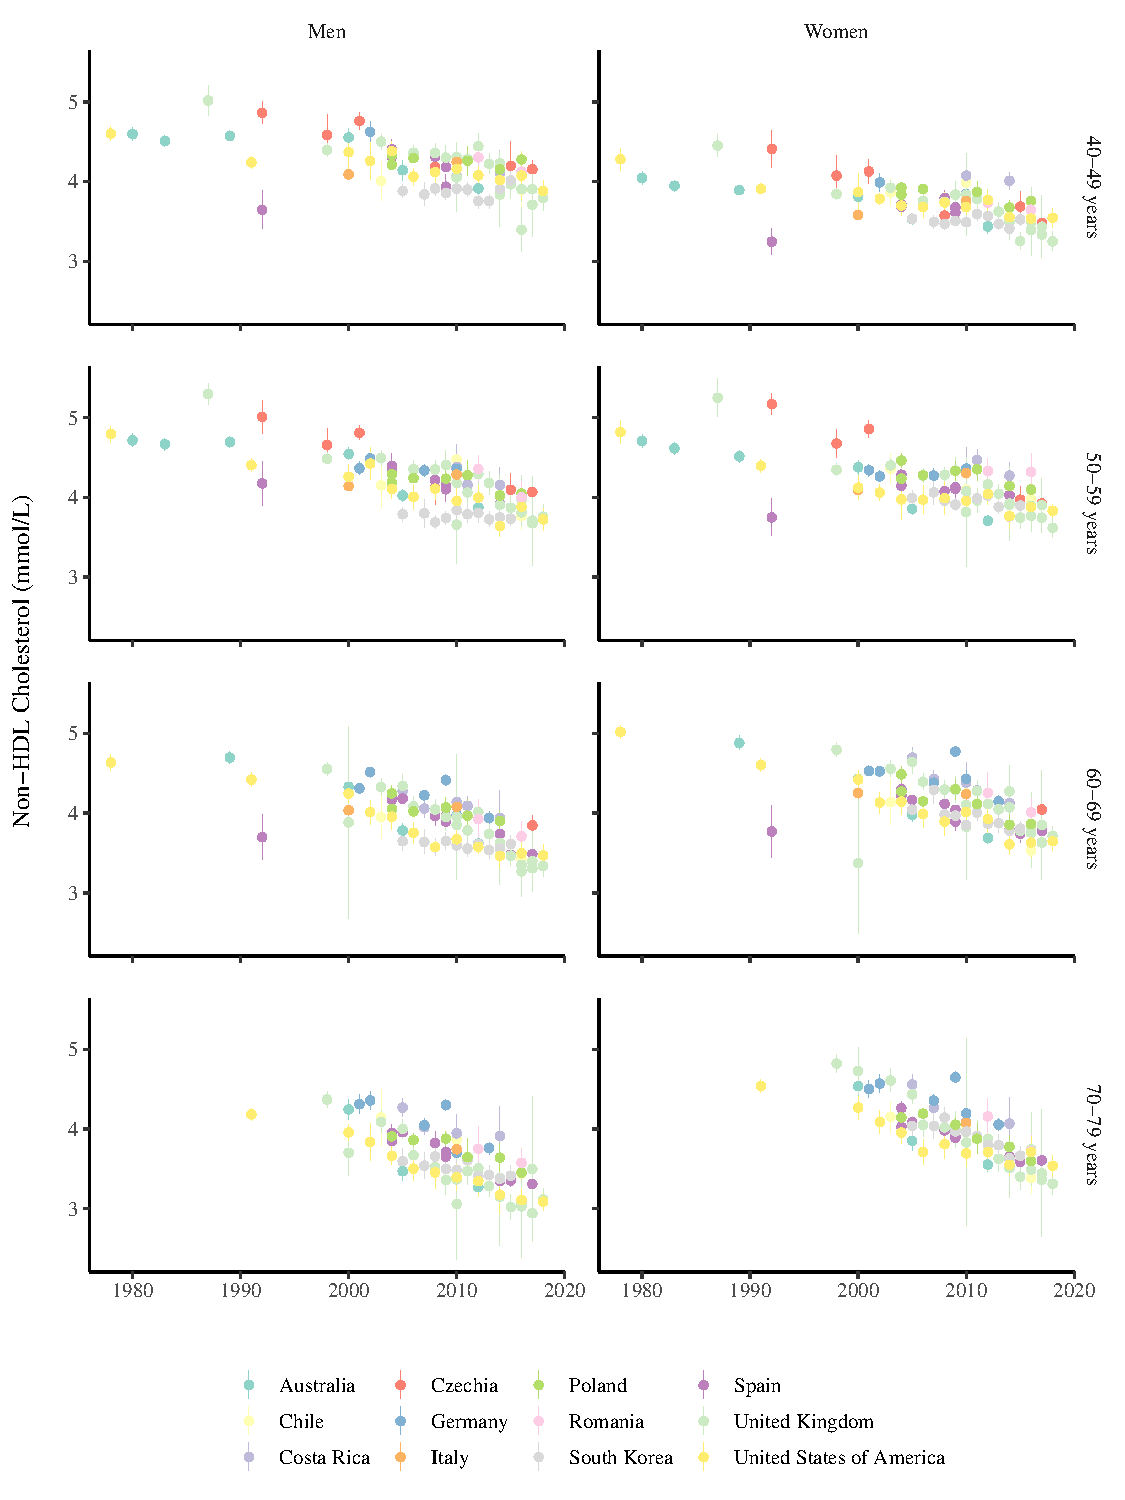
\includegraphics[width=\textwidth]{../3_figures/fig1_mean_chol.pdf}
 \caption{Trends in mean non-HDL serum cholesterol level, by country, sex, and age group.}
 \label{fig:mean_chol}
\end{figure}

\begin{figure}[hp]
    \centering
    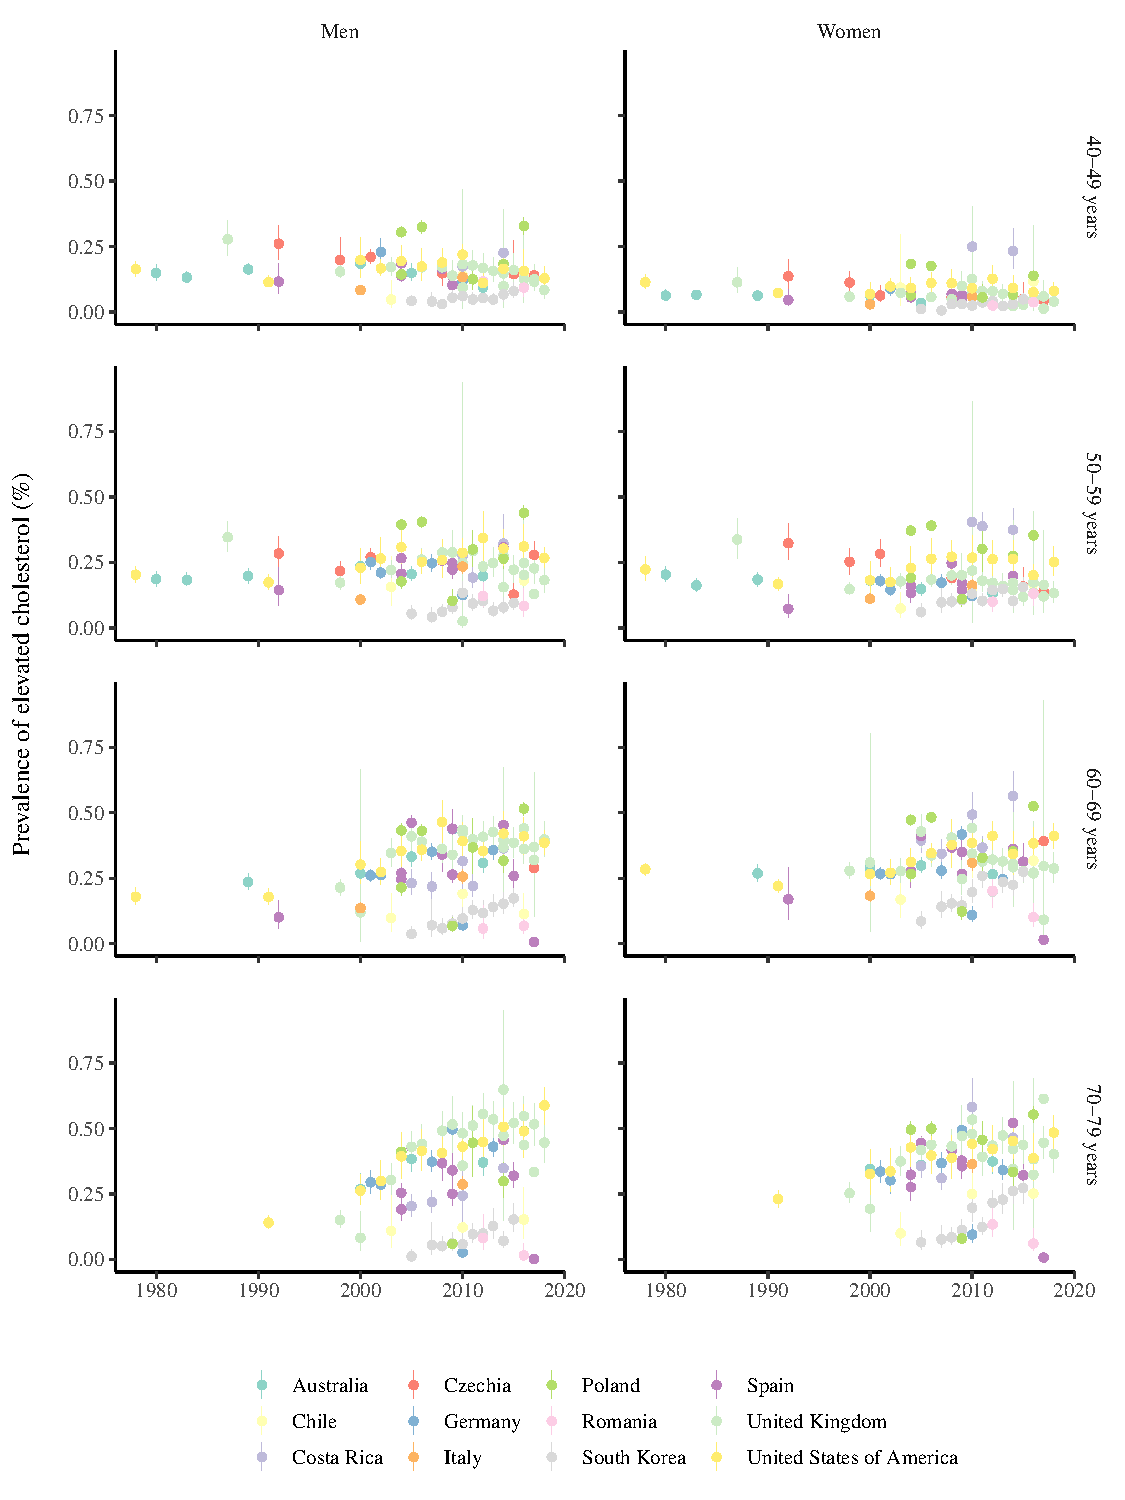
\includegraphics[width=\textwidth]{../3_figures/fig2_elevated.pdf}
    \caption{Trends in elevated serum cholesterol, by country, sex, and age group.}
    \label{fig:elevated}
\end{figure}

\begin{figure}[hp]
    \centering
    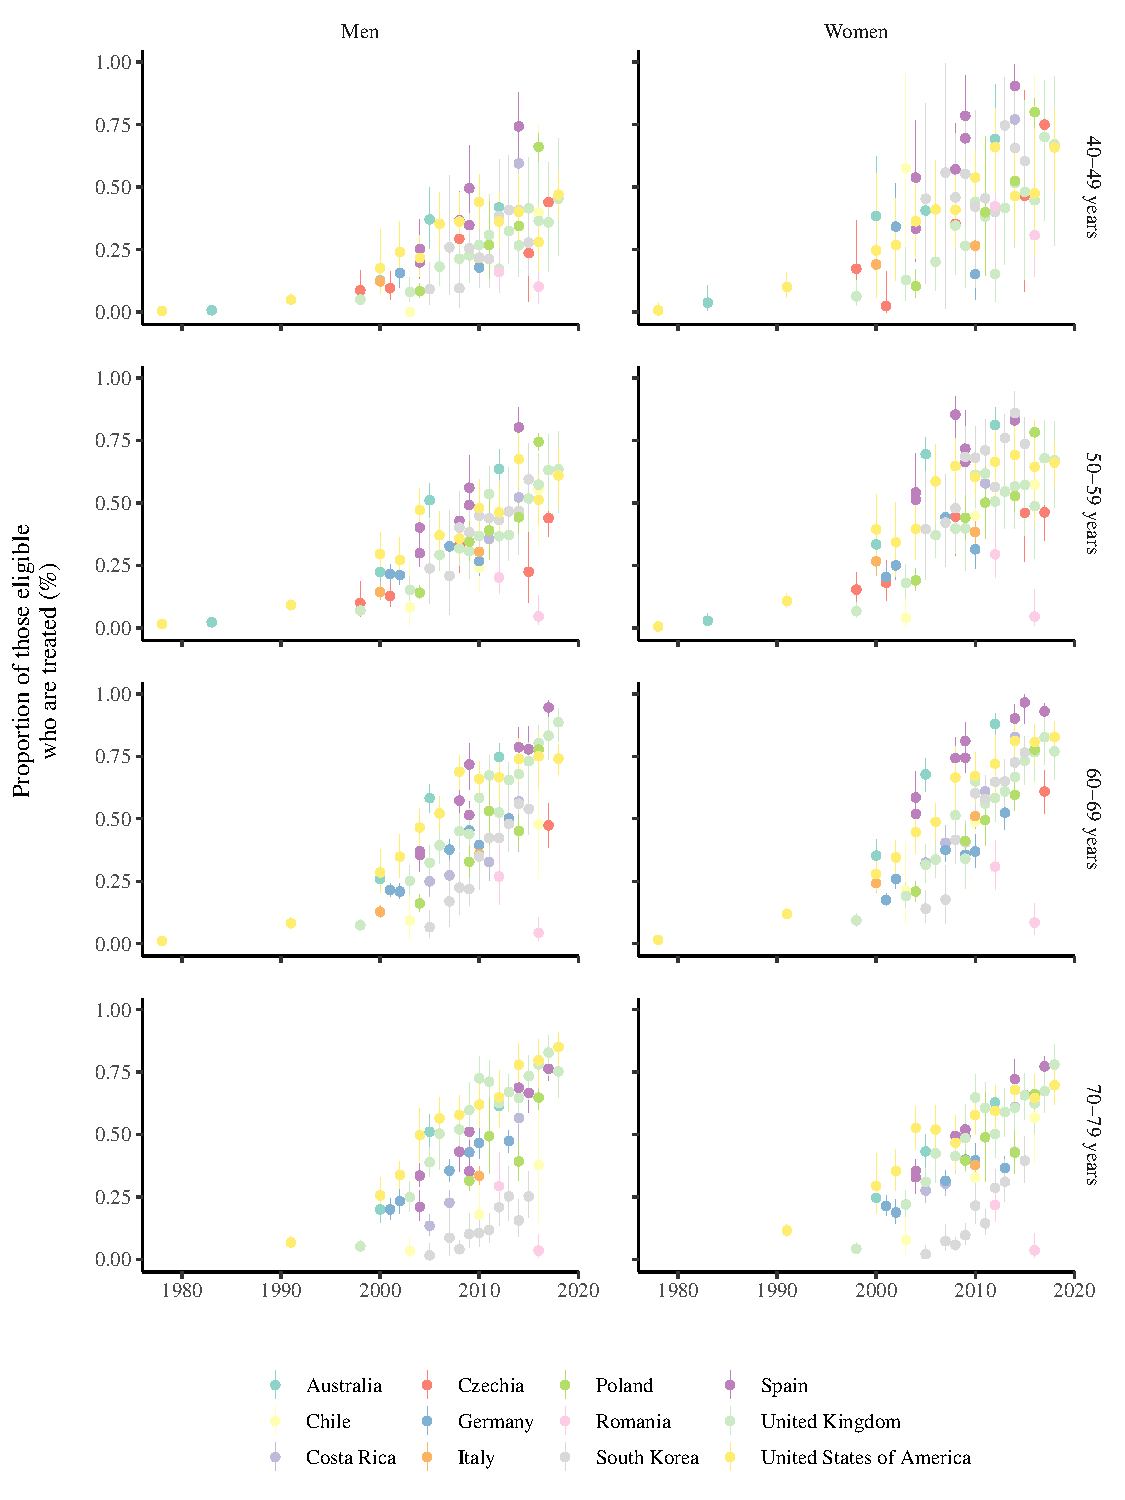
\includegraphics[width=\textwidth]{../3_figures/fig3_treated.pdf}
    \caption{Trends in treatment among people with elevated serum cholesterol, by country, sex, and age group.}
    \label{fig:treated}
\end{figure}

\clearpage
\setlength\bibsep{0pt}
\bibliographystyle{unsrt}
\bibliography{lipids}

\begin{appendix}
    \renewcommand{\thefigure}{A\arabic{figure}}
    \setcounter{figure}{0}
    
    \renewcommand{\thetable}{A\arabic{table}}
    \setcounter{table}{0}
    
%    \appendixwithtoc
    \newpage
    
    \section{Appendix} \label{sec:appendixa}
    \renewcommand{\thesection}{\Alph{section}}

    \subsection{Data sources}
    Using the NCDRisC database, we assembled data from 90 national health examination surveys completed between 1976 and 2018 in 12 high and middle-income countries: Australia, Chile, Costa Rica, Czech Republic, Germany, Italy, Poland, Romania, South Korea, Spain, United Kingdom, United States of America. These surveys included a lipid panel for a random sample of the general population. A list of surveys used and information about their design, including the age range and number of participants, whether LDL-C was calculated, and the devices used, is included in Table \ref{tab:data_sources}.
    
    \begin{landscape}
    \begin{singlespace}
        \begingroup\fontsize{7}{9}\selectfont

\begin{longtable}[t]{rlrrlllrr}
\caption{\label{tab:}Data sources from 12 high-income countries with laboratory lipid values}\\
\toprule
\multicolumn{5}{c}{ } & \multicolumn{2}{c}{Age range} & \multicolumn{2}{c}{Sample size} \\
\cmidrule(l{3pt}r{3pt}){6-7} \cmidrule(l{3pt}r{3pt}){8-9}
  & Country & Start & End & Survey name & Women & Men & Women & Men\\
\midrule
\endfirsthead
\caption[]{Data sources from 12 high-income countries with laboratory lipid values \textit{(continued)}}\\
\toprule
  & Country & Start & End & Survey name & Women & Men & Women & Men\\
\midrule
\endhead

\endfoot
\bottomrule
\endlastfoot
1 & Australia & 1980 & 1980 & Risk Factor Prevalence Study (RFPS) & 25-64 & 25-64 & 2756 & 2739\\
2 & Australia & 1983 & 1983 & Risk Factor Prevalence Study (RFPS) & 25-64 & 25-64 & 3732 & 3655\\
3 & Australia & 1989 & 1989 & Risk Factor Prevalence Study (RFPS) & 20-69 & 20-69 & 4611 & 4501\\
4 & Australia & 1999 & 2000 & The Australian Diabetes, Obesity and Lifestyle Study 1999-2000 (AusDiab) & 25+ & 25+ & 6138 & 5047\\
5 & Australia & 2004 & 2005 & The Australian Diabetes, Obesity and Lifestyle Study 2004-2005 (AusDiab) & 30+ & 30+ & 3444 & 2852\\
6 & Australia & 2012 & 2012 & The Australian Diabetes, Obesity and Lifestyle Study 2012 (AusDiab) & 37+ & 37+ & 2535 & 2046\\
\addlinespace
7 & Chile & 2003 & 2003 & Encuesta Nacional de Salud (ENS) & 17+ & 17+ & 1067 & 909\\
8 & Chile & 2009 & 2010 & Encuesta Nacional de Salud (ENS) & 15+ & 15+ & 1600 & 1122\\
9 & Chile & 2016 & 2017 & Encuesta Nacional de Salud (ENS) & 15+ & 15+ & 2349 & 1366\\
\addlinespace
10 & Costa Rica & 2004 & 2006 & Costa Rican Longevity and Healthy Aging Study Pre-1945 Cohort Wave 1 (CRELES) & 60+ & 60+ & 1448 & 1208\\
11 & Costa Rica & 2006 & 2008 & Costa Rican Longevity and Healthy Aging Study Pre-1945 Cohort Wave 2 (CRELES) & 62+ & 62+ & 1215 & 1018\\
12 & Costa Rica & 2010 & 2011 & Costa Rican Longevity and Healthy Aging Study 1945-1955 Cohort Wave 1 (CRELES) & 54-66 & 54-66 & 1590 & 1029\\
13 & Costa Rica & 2010 & 2010 & Costa Rican National Cardiovascular Risk Factors Survey, 2010 (CRFS) & 20+ & 20+ & 1937 & 725\\
14 & Costa Rica & 2014 & 2014 & Costa Rican National Cardiovascular Risk Factors Survey, 2014 (CRFS) & 20+ & 20+ & 1671 & 706\\
\addlinespace
15 & Czech Republic & 1992 & 1992 & MONICA, Czech Republic & 25-64 & 25-64 & 1189 & 1127\\
16 & Czech Republic & 1997 & 1998 & Czech post-MONICA (postMONICA) & 25-64 & 25-64 & 1664 & 1527\\
17 & Czech Republic & 2000 & 2001 & Czech post-MONICA (postMONICA) & 25-64 & 25-64 & 1661 & 1612\\
18 & Czech Republic & 2006 & 2009 & Czech post-MONICA (postMONICA) & 25-64 & 25-64 & 1860 & 1718\\
19 & Czech Republic & 2014 & 2015 & European Heath Examination Survey (EHES) & 25-64 & 25-64 & 681 & 472\\
20 & Czech Republic & 2015 & 2018 & MONICA & 25-65 & 25-65 & 1361 & 1239\\
\addlinespace
21 & Germany & 2000 & 2002 & ESTHER & 50-75 & 50-75 & 5270 & 4340\\
22 & Germany & 2000 & 2003 & Heinz Nixdorf Recall Study (HNRS) & 45-75 & 45-75 & 2402 & 2381\\
23 & Germany & 2005 & 2008 & Heinz Nixdorf Recall Study (HNRS) & 50-80 & 50-80 & 2082 & 2045\\
24 & Germany & 2008 & 2011 & ESTHER & 58-84 & 58-84 & 2488 & 2082\\
25 & Germany & 2008 & 2012 & Study of Health in Pomerania, second cohort (SHIP-TREND) & 20-79 & 20-79 & 2233 & 2098\\
26 & Germany & 2011 & 2014 & Heinz Nixdorf Recall Study (HNRS) & 56-85 & 56-85 & 1557 & 1492\\
\addlinespace
27 & Italy & 1998 & 2002 & Osservatorio Epidemiologico Cardiovascolare (OEC) & 35-74 & 35-74 & 4705 & 4831\\
28 & Italy & 2008 & 2012 & Osservatorio Epidemiologico Cardiovascolare/Health Examination Survey (OEC) & 35-80 & 35-80 & 4302 & 4331\\
\addlinespace
29 & Poland & 2003 & 2005 & National Multicenter Health Survey in Poland. Project WOBASZ & 20-74 & 20-74 & 6809 & 6119\\
30 & Poland & 2004 & 2004 & LIPIDOGRAM2004 Study & 30+ & 30+ & 9920 & 6672\\
31 & Poland & 2006 & 2006 & LIPIDOGRAM2006 Study & 32+ & 32+ & 10640 & 6440\\
32 & Poland & 2007 & 2011 & Medical, psychological and socioeconomic aspects of aging in Poland (PolSenior) & 55+ & 55+ & 2306 & 2427\\
33 & Poland & 2011 & 2011 & NATPOL & 18-79 & 18-79 & 1213 & 1147\\
34 & Poland & 2013 & 2014 & National Multicenter Health Survey in Poland. Project WOBASZ II & 20+ & 20+ & 3233 & 2633\\
35 & Poland & 2015 & 2016 & LIPIDOGRAM2015 \& LIPIDOGEN2015 Study & 18+ & 18+ & 8688 & 5032\\
\addlinespace
36 & Romania & 2011 & 2012 & SEPHAR II & 18-80 & 18-80 & 1037 & 931\\
37 & Romania & 2015 & 2016 & SEPHAR III & 18-80 & 18-80 & 1033 & 935\\
\addlinespace
38 & South Korea & 2005 & 2005 & Korea National Health and Nutrition Examination Survey (KNHANES) & 10+ & 10+ & 3475 & 2755\\
39 & South Korea & 2007 & 2007 & Korea National Health and Nutrition Examination Survey (KNHANES) & 10+ & 10+ & 1813 & 1388\\
40 & South Korea & 2008 & 2008 & Korea National Health and Nutrition Examination Survey (KNHANES) & 10+ & 10+ & 4142 & 3203\\
41 & South Korea & 2009 & 2009 & Korea National Health and Nutrition Examination Survey (KNHANES) & 10+ & 10+ & 4438 & 3606\\
42 & South Korea & 2010 & 2010 & Korea National Health and Nutrition Examination Survey (KNHANES) & 10+ & 10+ & 3661 & 2976\\
43 & South Korea & 2011 & 2011 & Korea National Health and Nutrition Examination Survey (KNHANES) & 10+ & 10+ & 3670 & 2888\\
44 & South Korea & 2012 & 2012 & Korea National Health and Nutrition Examination Survey (KNHANES) & 10+ & 10+ & 3461 & 2691\\
45 & South Korea & 2013 & 2013 & Korea National Health and Nutrition Examination Survey (KNHANES) & 10+ & 10+ & 3219 & 2635\\
46 & South Korea & 2014 & 2014 & Korea National Health and Nutrition Examination Survey (KNHANES) & 10+ & 10+ & 3025 & 2365\\
47 & South Korea & 2015 & 2015 & Korea National Health and Nutrition Examination Survey (KNHANES) & 10+ & 10+ & 3080 & 2568\\
\addlinespace
48 & Spain & 1991 & 1993 & Cardiovascular Risk Factors Survey in Murcia (CVDRF) & 18-69 & 18-69 & 1268 & 1151\\
49 & Spain & 2003 & 2005 & Registre Gironi del Cor (REGICOR) & 35-79 & 35-79 & 3280 & 2951\\
50 & Spain & 2004 & 2006 & PREVICTUS & 60+ & 60+ & 3834 & 3350\\
51 & Spain & 2004 & 2004 & Cardiovascular Risk Study in Castilla y León (RECCyL) & 15+ & 15+ & 2069 & 1897\\
52 & Spain & 2007 & 2009 & Harmonizing Equation of Risk in Mediterraneon countries EXtremadura (HERMEX) & 25-79 & 25-79 & 1498 & 1297\\
53 & Spain & 2008 & 2010 & Study on Nutrition and Cardiovascular Risk in Spain (ENRICA) & 18+ & 18+ & 6858 & 6193\\
54 & Spain & 2009 & 2009 & Cardiovascular Risk Study in Castilla y León (RECCyL) & 20+ & 20+ & 1572 & 1291\\
55 & Spain & 2014 & 2014 & Cardiovascular Risk Study in Castilla y León (RECCyL) & 20+ & 20+ & 1509 & 1220\\
56 & Spain & 2015 & 2015 & Study on Nutrition and Cardiovascular Risk in Spain (ENRICA) & 65+ & 65+ & 770 & 704\\
\addlinespace
57 & United Kingdom & 1986 & 1987 & Dietary and Nutritional Survey of British Adults 1986-1987 (DNS) & 16-64 & 16-64 & 937 & 936\\
58 & United Kingdom & 1998 & 1998 & Health Survey for England (HSE) & 16+ & 16+ & 5565 & 5000\\
59 & United Kingdom & 2003 & 2003 & Health Survey for England (HSE) & 16+ & 16+ & 4460 & 3814\\
60 & United Kingdom & 2005 & 2005 & Health Survey for England (HSE) & 65+ & 65+ & 1190 & 1008\\
61 & United Kingdom & 2006 & 2006 & Health Survey for England (HSE) & 16+ & 16+ & 4061 & 3409\\
62 & United Kingdom & 2008 & 2008 & Health Survey for England (HSE) & 16+ & 16+ & 3922 & 3348\\
63 & United Kingdom & 2008 & 2012 & National Diet and Nutrition Survey (NDNS) & 10+ & 10+ & 1266 & 1008\\
64 & United Kingdom & 2009 & 2009 & Health Survey for England (HSE) & 16+ & 16+ & 1227 & 1075\\
65 & United Kingdom & 2010 & 2010 & Health Survey for England (HSE) & 16+ & 16+ & 2158 & 1720\\
66 & United Kingdom & 2011 & 2011 & Health Survey for England (HSE) & 16+ & 16+ & 2201 & 1738\\
67 & United Kingdom & 2012 & 2012 & Health Survey for England (HSE) & 16+ & 16+ & 2192 & 1745\\
68 & United Kingdom & 2013 & 2013 & Health Survey for England (HSE) & 16+ & 16+ & 2438 & 2080\\
69 & United Kingdom & 2013 & 2014 & National Diet and Nutrition Survey (NDNS) & 10+ & 10+ & 520 & 386\\
70 & United Kingdom & 2014 & 2014 & Health Survey for England (HSE) & 16+ & 16+ & 2085 & 1816\\
71 & United Kingdom & 2015 & 2015 & Health Survey for England (HSE) & 16+ & 16+ & 2130 & 1777\\
72 & United Kingdom & 2015 & 2016 & National Diet and Nutrition Survey (NDNS) & 10+ & 10+ & 485 & 391\\
73 & United Kingdom & 2016 & 2016 & Health Survey for England (HSE) & 16+ & 16+ & 2083 & 1682\\
74 & United Kingdom & 2016 & 2017 & National Diet and Nutrition Survey (NDNS) & 10+ & 10+ & 204 & 174\\
75 & United Kingdom & 2017 & 2017 & Health Survey for England (HSE) & 16+ & 16+ & 2160 & 1711\\
76 & United Kingdom & 2018 & 2018 & Health Survey for England (HSE) & 16+ & 16+ & 1947 & 1600\\
\addlinespace
77 & United States of America & 1976 & 1980 & US NHANES II & 20-74 & 20-74 & 6245 & 5601\\
78 & United States of America & 1988 & 1994 & US NHANES III & 10+ & 10+ & 10275 & 9408\\
79 & United States of America & 1999 & 2000 & US NHANES 1999-2000 & 10+ & 10+ & 3123 & 3150\\
80 & United States of America & 2001 & 2002 & US NHANES 2001-2002 & 10+ & 10+ & 3402 & 3496\\
81 & United States of America & 2003 & 2004 & US NHANES 2003-2004 & 10+ & 10+ & 3202 & 3361\\
82 & United States of America & 2005 & 2006 & US NHANES 2005-2006 & 10+ & 10+ & 3128 & 3302\\
83 & United States of America & 2007 & 2008 & US NHANES 2007-2008 & 10+ & 10+ & 3333 & 3367\\
84 & United States of America & 2009 & 2010 & US NHANES 2009-2010 & 10+ & 10+ & 3599 & 3558\\
85 & United States of America & 2011 & 2012 & US NHANES 2011-2012 & 10+ & 10+ & 3131 & 3155\\
86 & United States of America & 2013 & 2014 & US NHANES 2013-2014 & 10+ & 10+ & 3535 & 3350\\
87 & United States of America & 2015 & 2016 & US NHANES 2015-2016 & 10+ & 10+ & 3320 & 3218\\
88 & United States of America & 2017 & 2018 & US NHANES 2017-2018 & 10+ & 10+ & 3153 & 3011\\*
\end{longtable}
\endgroup{}

        \label{tab:data_sources}
    \end{singlespace}
    \end{landscape}

    \subsection{Exlusion criteria}

    \begin{figure}[H]
        \centering
        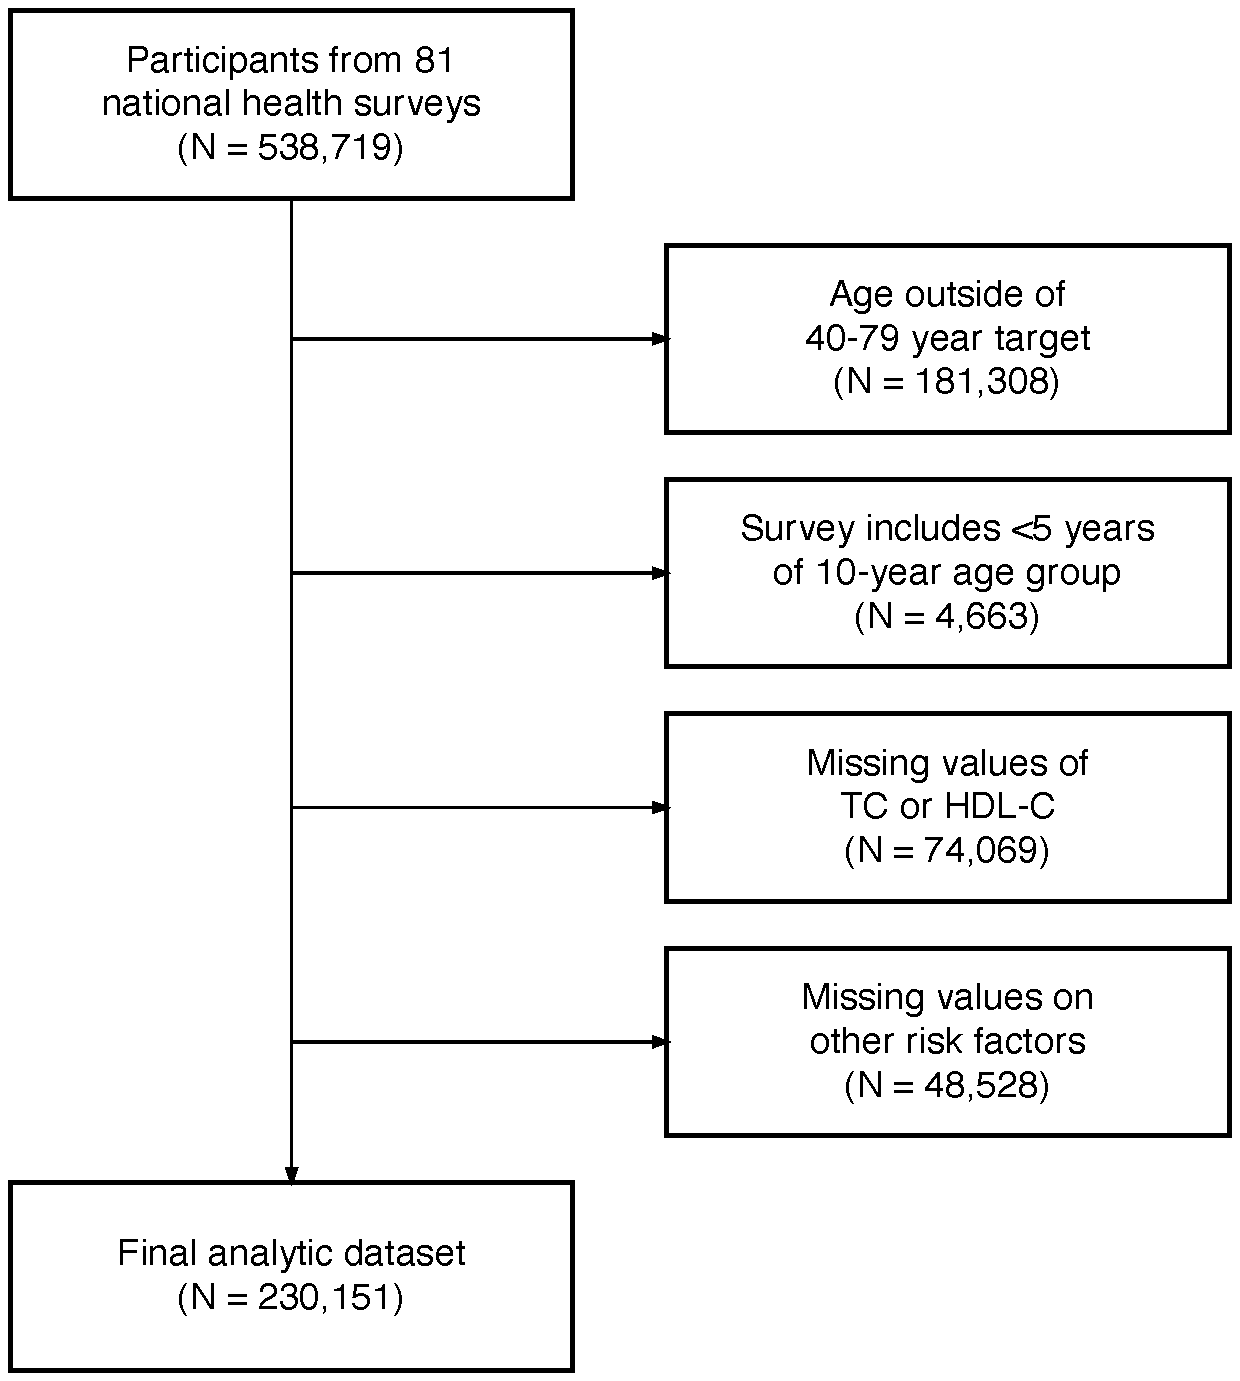
\includegraphics[width=0.5\linewidth]{../3_figures/figS_STROBE.pdf}
        \caption{Exclusion criteria.}
        \label{fig:exclusion}
    \end{figure}


    \subsection{Data cleaning}
    Given the heterogeneity in the data collection and cleaning across surveys, we implemented a secondary data cleaning protocol and applied to the pooled data from all 90 surveys. The basic steps were as follows, we evaluated:
    \begin{enumerate}
        \item univariate plausibility ranges
        \item multivariate plausibility constraints
        \item multivariate outlier detection
    \end{enumerate}

    \subsubsection{Univariate plausibility ranges}
    We removed values for certain laboratory and examination measurements that were outside the range of biological plausibility, as determined by expert consensus. Table \ref{tab:plausibility} below shows the plausiblity ranges used for each variable as well as the number and fraction of values removed.

    \begin{table}[h]
        \centering
        \caption{Univariate plausibility ranges for select variables from national surveys.}
        \begin{tabular}{lcc}
            \hline
            Variable & Ages & Plausibility range \\
            \hline
            height (cm) & 5 to 9 years & 60 - 180 \\
            height (cm) & 10 to 14 years & 80 - 200 \\
            height (cm) & $\geq$15 years & 100 - 250 \\
            weight (kg) & 5 to 9 years & 5 - 90 \\
            weight (kg) & 10 to 14 years & 8 - 150 \\
            weight (kg) & $\geq$15 years & 12 - 300 \\
            BMI (kg/m$^2$) & 5 to 9 years & 6 - 40 \\
            BMI (kg/m$^2$) & 10 to 14 years & 8 - 60 \\
            BMI (kg/m$^2$) & $\geq$15 years & 10 - 80 \\
            SBP (mmHg) & all & 70 - 270 \\
            DBP (mmHg) & all & 30 - 150 \\
            TC (mmol/L) & all & 1.75 - 20 \\
            LDL (mmol/L) & all & 0.5 - 10 \\
            HDL (mmol/L) & all & 0.4 - 5 \\
            Triglycerides (mmol/L) & all & 0.2-20 \\
            \hline
        \end{tabular}
        \label{tab:plausibility}
    \end{table}

    \subsubsection{Multivariate plausibility constraints}
    The following constraints are applied after removing data outside the plausibility ranges listed above:
    \begin{itemize}
        \item SBP $>$ DBP (before calculating average BP) 
        \item TC $>$ LDL 
        \item TC $>$ HDL
        \item TC – (LDL + HDL) $\geq$ margin of error
    \end{itemize}

* “margin of error” is determined by using the Cholesterol Reference Method Laboratory Network permitted measurement error limits for TC (8.9\%), HDL (13\%) and LDL (12\%) as follows:
-	Calculate errors in worst case scenario, i.e., TC underestimated, and HDL/LDL overestimated, each by the largest error permitted.
-	The limit of errors by quartiles of TC using US NHANES data

    \subsubsection{Multivariate outlier detection}

    For each pair listed above:
-	Compute the Mahalanobis of distance of all the data points after normalisation.
-	Exclude points with distance larger than 40.08, which is the quantile of chi2 distribution equivalent to 6SD for normal distribution.

Note: The same cut-off is applied to all pairs. This cut-off may change when applying the procedure to the whole NCD-RisC database.

\begin{figure}[H]
    \centering
    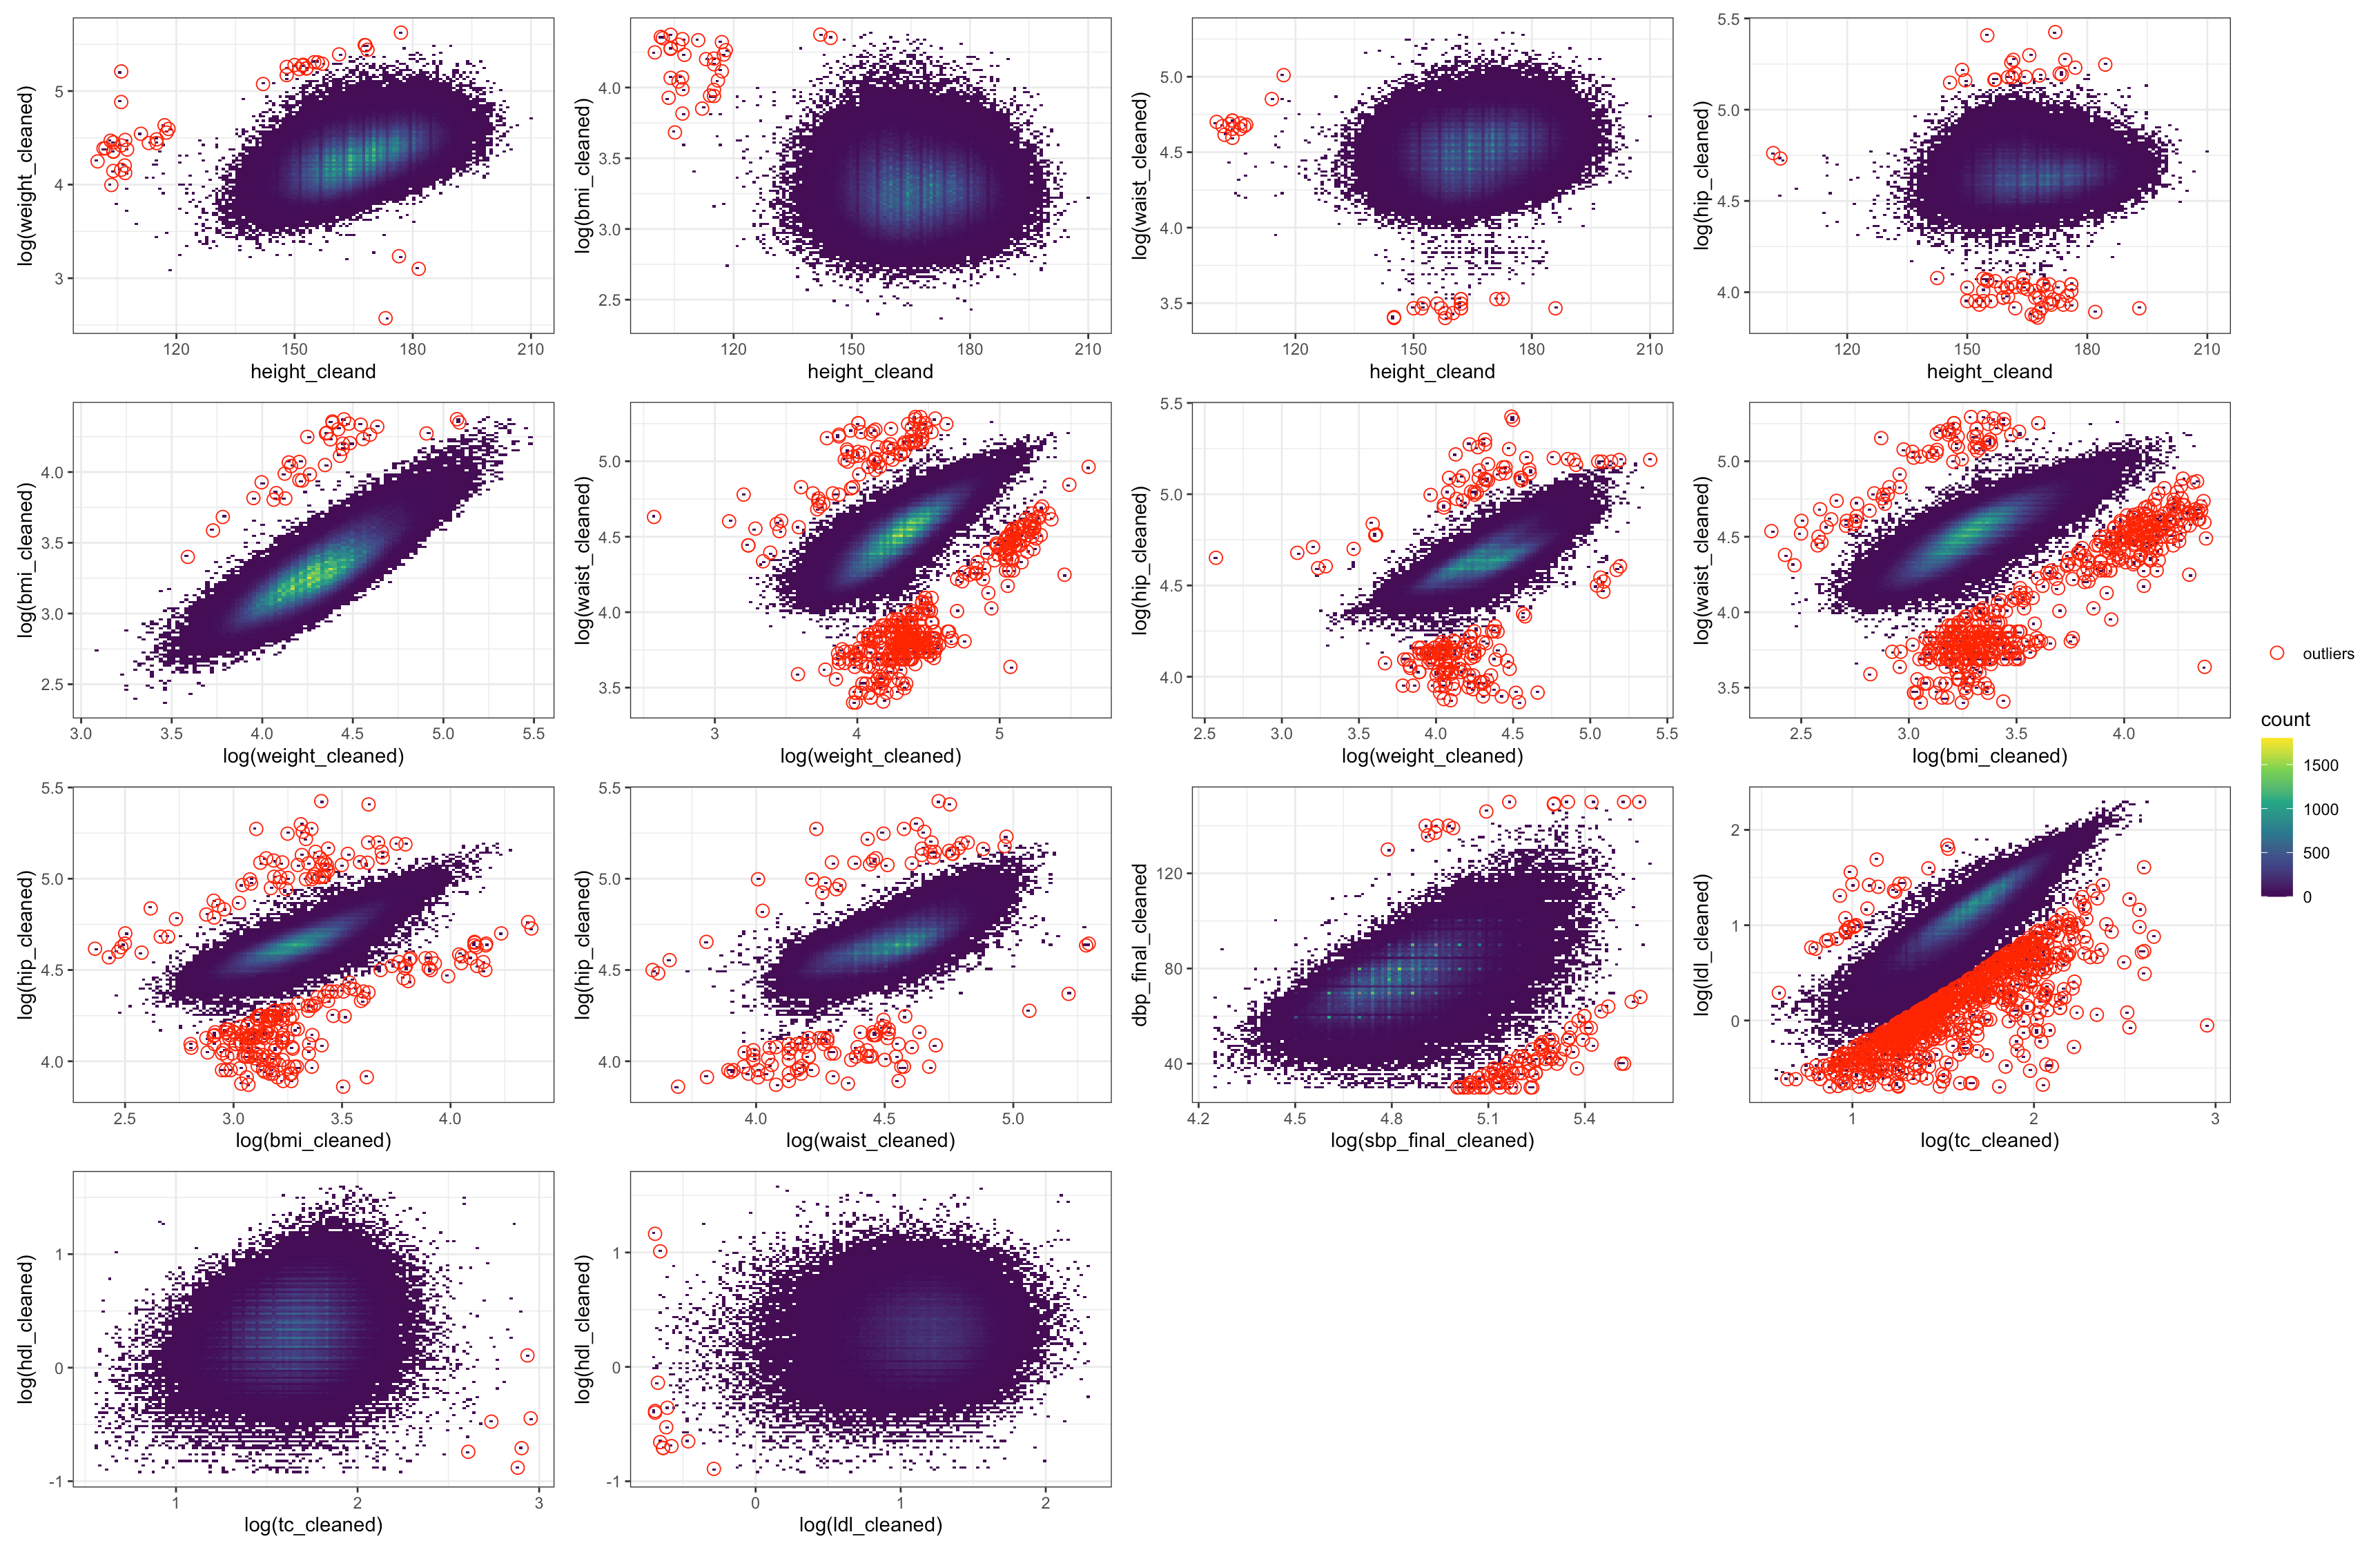
\includegraphics[width = \linewidth]{../3_figures/mahalanobis.png}
    \caption{Pairwise outliers based on Mahalanobis distance}
    \label{fig:pairs}
\end{figure}

    \subsection{Cholesterol Treatment Guidelines}

    We compiled a list of cholesterol treatment guidelines from official sources that have been published and discussed in the academic literature. Most of these come from a review conducted by the World Heart Foundation in 2019. They will be used, possibly, as criteria for determining who should be on treatment in assembled surveys. Note that many of these same sources have guidance about control as well (i.e. ideal reductions in LDL or absolute level attained while on treatment). Table \ref{tab:guidelines} below summarizes the specific treatment guidance from the US, Europe, the UK, Canada, China, Brazil, South Africa, and the WHO. 

    \begin{table}[H]
        \centering
        \tiny{
        \begin{threeparttable}
        \begin{tabular}{llll}
            \toprule
            Source & Year & Treatment recommendation & Goal of therapy\\
            \midrule  
            %  \hline
            NHLBI NCEP ATP III \cite{noauthor_third_2002} & 2013 & LDL $\geq 100$ mg/dL and 10-year risk\tnote{*} \hspace{1pt}  $\geq$ 20\%  & LDL $<$ 100 mg/dL \\
            & & LDL $\geq 130$ mg/dL and 10-year risk\tnote{*} \hspace{1pt}  $\geq$ 10\% (2+ risk factors) & LDL $<$ 130 mg/dL  \\
            & & LDL $\geq 160$ mg/dL and 10-year risk\tnote{*} \hspace{1pt}  $<$ 10\% (2+ risk factors) & LDL $<$ 130 mg/dL  \\
            & & LDL $\geq 190$ mg/dL (0-1 risk factors) & LDL $<$ 160 mg/dL \\
            & & & \\
            %  \hline
            AHA/ACC Statement \cite{grundy_scott_m_2018_2019} & 2018 & LDL $\geq 190$ mg/dL (severe hypercholesterolemia) & LDL $<$ 100 mg/dL \\
            & & LDL $\geq 70$ mg/dL and 10-year risk\tnote{*} \hspace{1pt}  $\geq$ 7.5\%  & LDL reduced 30\% to 49\%\\
            & & LDL $\geq 70$ mg/dL and 10-year risk\tnote{*} \hspace{1pt}  $\geq$ 20\% & LDL reduced $\geq$ 50\%\\
            & & LDL $\geq 70$ mg/dL and diabetes mellitus & LDL reduced $\geq$ 50\% \\
            & & & \\
            ESC/EAS Guidelines \cite{mach_2019_2020} & 2019 & LDL $\geq 70$ mg/dL and 10-year risk\tnote{\textdagger} \hspace{1pt} $\geq$ 10\% (very-high) & LDL reduced $\geq$ 50\% or $<$ 55 mg/dL \\
            & & LDL $\geq 100$ mg/dL and 10-year risk\tnote{\textdagger} \hspace{1pt}  $\geq$ 5\% (high) & LDL reduced $\geq$ 50\% or $<$ 70 mg/dL \\
            & & LDL $\geq 190$ mg/dL and 10-year risk\tnote{\textdagger} \hspace{1pt}  $\geq$ 1\% (moderate) & LDL $<$ 100 mg/dL \\
            & & LDL $\geq 190$ mg/dL and 10-year risk\tnote{\textdagger} \hspace{1pt} $<$ 1\% (low) & LDL $<$ 116 mg/dL \\
            & & & \\
            NICE Guidelines \cite{rabar_lipid_2014} & 2014 & 10-year risk\tnote{\ddag} \hspace{1pt} $\geq$ 10\% or CKD &  \\
            & & diabetes mellitus (type-2) and 10-year risk\tnote{\ddag} \hspace{1pt} $\geq$ 10\% &  \\
            & & diabetes mellitus (type-1), $>$40 years-old, duration $>$10 years &  \\
            & & & \\
            CCS Guidelines \cite{anderson_2012_2013} & 2012 & LDL $\geq 75$ mg/dL and 10-year risk\tnote{\S} \hspace{1pt} $\geq$ 20\% & LDL $<$ 75 mg/dL \\
            & & LDL $\geq 130$ mg/dL and 10-year risk\tnote{\S} \hspace{1pt}  $\geq$ 10\% & LDL $<$ 130 mg/dL \\
            & & LDL $\geq 130$ mg/dL and 10-year risk\tnote{\S} \hspace{1pt}  $\geq$ 5\% (optional) & LDL $<$ 190 mg/dL \\
            & & LDL $\geq 190$ mg/dL and 10-year risk\tnote{\S} \hspace{1pt} $<$ 1\% & LDL $<$ 190 mg/dL \\
            & & & \\
            China Guidelines \cite{anderson_2012_2013} & 2016 & 10-year risk\tnote{$||$} \hspace{1pt} $\geq$ 10\% & LDL $<$ 130 mg/dL \\
            & & 10-year risk\tnote{$||$} \hspace{1pt} $\geq$ 5\% & LDL $<$ 130 mg/dL \\
            & & diabetes mellitus and LDL $\geq 70$ mg/dL or TC $\geq 120$ & LDL $<$ 100 mg/dL \\
            & & LDL $\geq 190$ mg/dL or TC $\geq 280$ & LDL $<$ 100 mg/dL \\
            & & & \\
            Brazil Guidelines \cite{anderson_2012_2013} & 2013 & 10-year risk\tnote{\S} \hspace{1pt} $\geq$ 10\% (women) $\geq$ 20\% (men) & LDL $<$ 100 mg/dL \\
            & & diabetes mellitus or CKD or FH & LDL $<$ 70 mg/dL \\
            & & & \\
            South Africa Guidelines \cite{anderson_2012_2013} & 2012 & 10-year risk\tnote{\S} \hspace{1pt} $\geq$ 30\% (very high) & LDL $<$ 70 mg/dL \\
            & & LDL $\geq 100$ mg/dL and 10-year risk\tnote{\S} \hspace{1pt}  $\geq$ 15\% (high) & LDL $<$ 100 mg/dL \\
            & & diabetes mellitus or CKD or FH & LDL $<$ 70 mg/dL \\
            & & & \\
            WHO Guidelines \cite{anderson_2012_2013} & 2007 & TC $\geq$ 320 mg/dL or LDL $\geq$ 240 mg/dL or TC/HDL ratio $>$ 8 & LDL $<$ 77 mg/dL or TC $<$ 152 mg/dL \\
            & & diabetes mellitus & LDL $<$ 77 mg/dL or TC $<$ 152 mg/d  \\
            & & 10-year risk\tnote{\P} \hspace{1pt} $\geq$ 30\% & LDL $<$ 77 mg/dL or TC $<$ 152 mg/dL \\
            & & LDL $\geq 115$ mg/dL or TC $\geq 193$ mg/dL and 10-year risk\tnote{\P} \hspace{1pt}  $\geq$ 20\% & LDL $<$ 100 mg/dL \\
            \bottomrule
        \end{tabular}
        \begin{tablenotes}
            \item[*] Based on Pooled Cohort Equations
            \item[\textdagger] Based on SCORE
            \item[\ddag] Based on QRISK2
            \item[\S] Based on Framingham Risk Score
            \item[$||$] Based on CMCS re-callibration
            \item[\P] Based on WHO/ISH risk charts
        \end{tablenotes}
        \end{threeparttable}
        }
        \caption{Cholesterol treatment guidelines and recommendations for primary prevention.}
        \label{tab:guidelines}
    \end{table}

    \subsection{Calibrating Non-HDL-C to LDL-C}


    \begin{figure}[H]
    \centering
    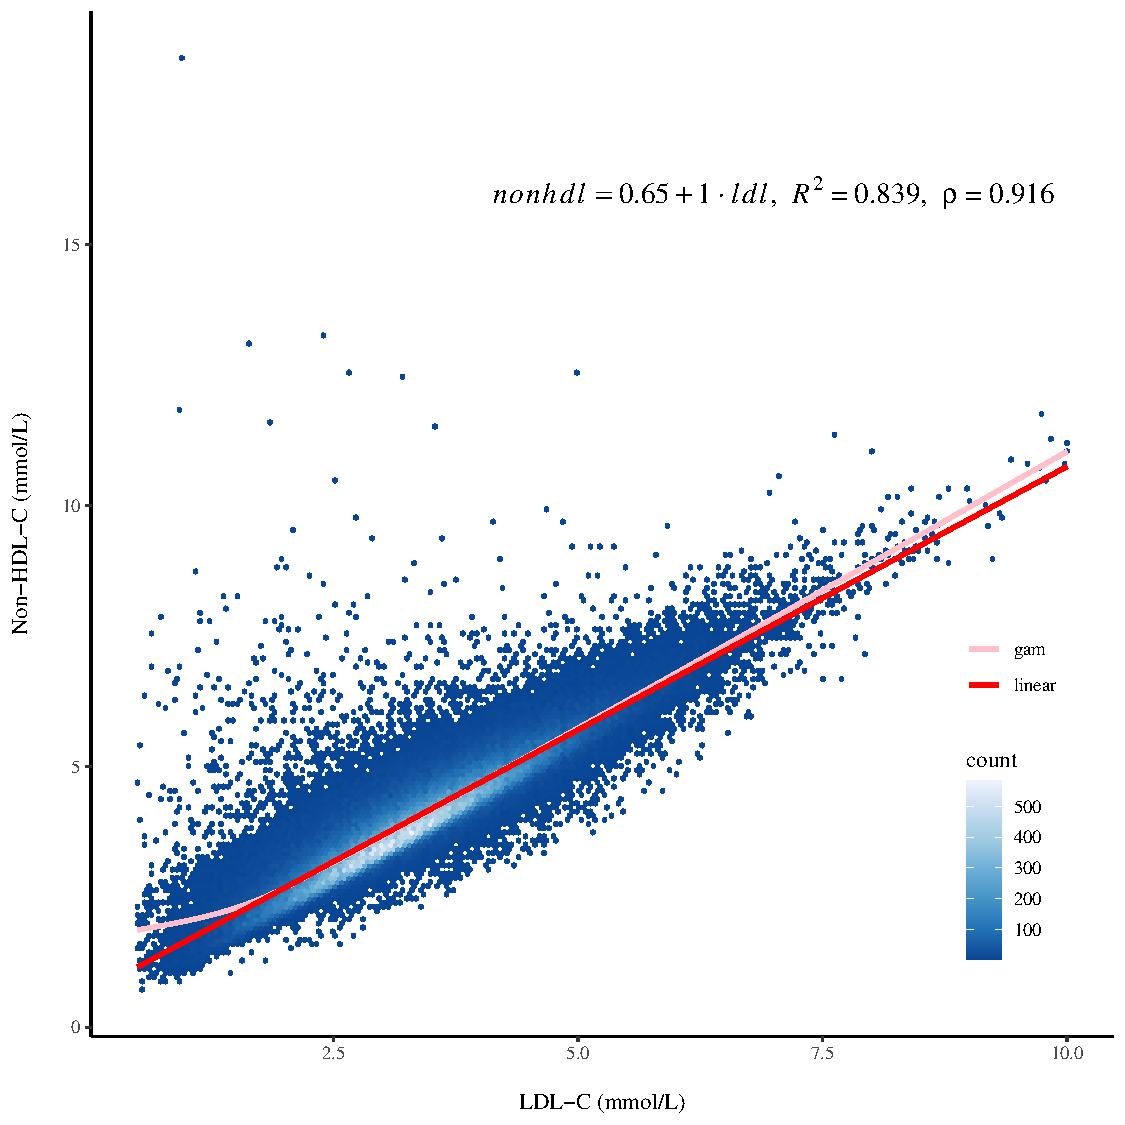
\includegraphics[width=\textwidth]{../3_figures/figS1_calibration.pdf}
    \caption{Placeholder}
    \label{fig:placeholder}
    \end{figure}
    
    \subsection{Variable definitions}
    
    \subsection{Sensitivity analyses}

    \subsection{Linear trends}

    \begin{figure}[H]
        \centering
        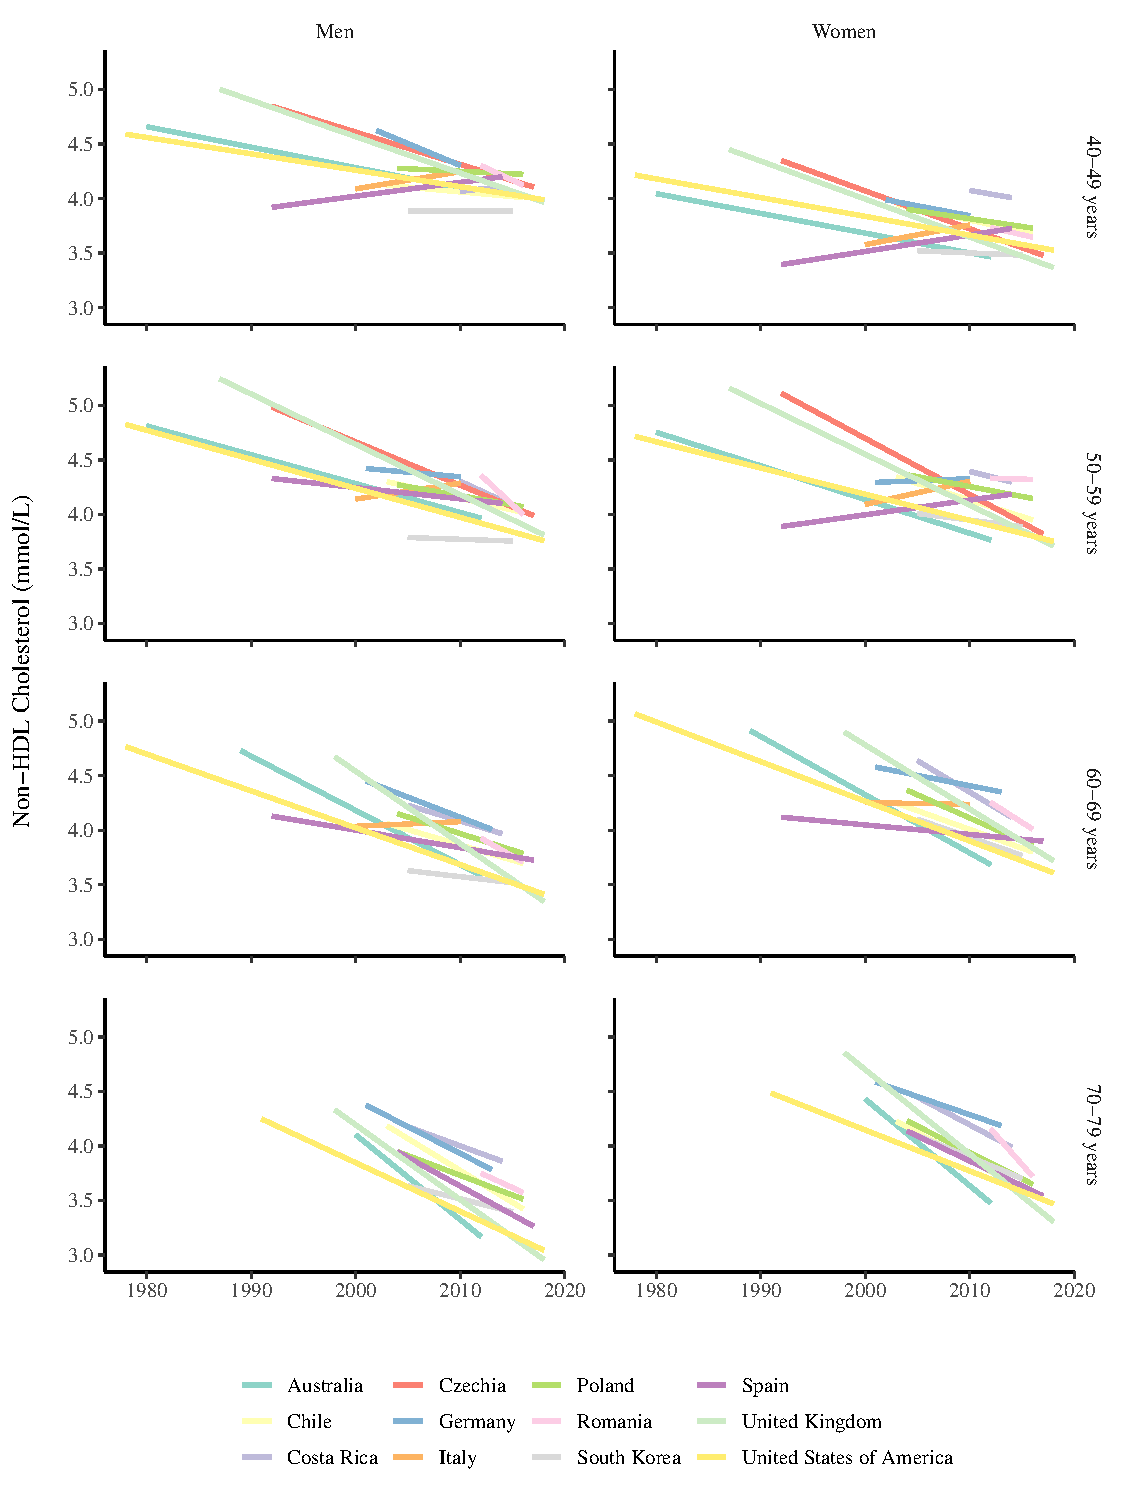
\includegraphics[width=\linewidth]{../3_figures/figS_mean_chol_trends.pdf}
        \caption{Linear trends in mean Non-HDL serum cholesterol level by country, age, and sex.}
        \label{fig:trends}
    \end{figure}


    \subsection{Country-by-country results}

    \begin{landscape}
        \begin{figure}[H]
            \centering
            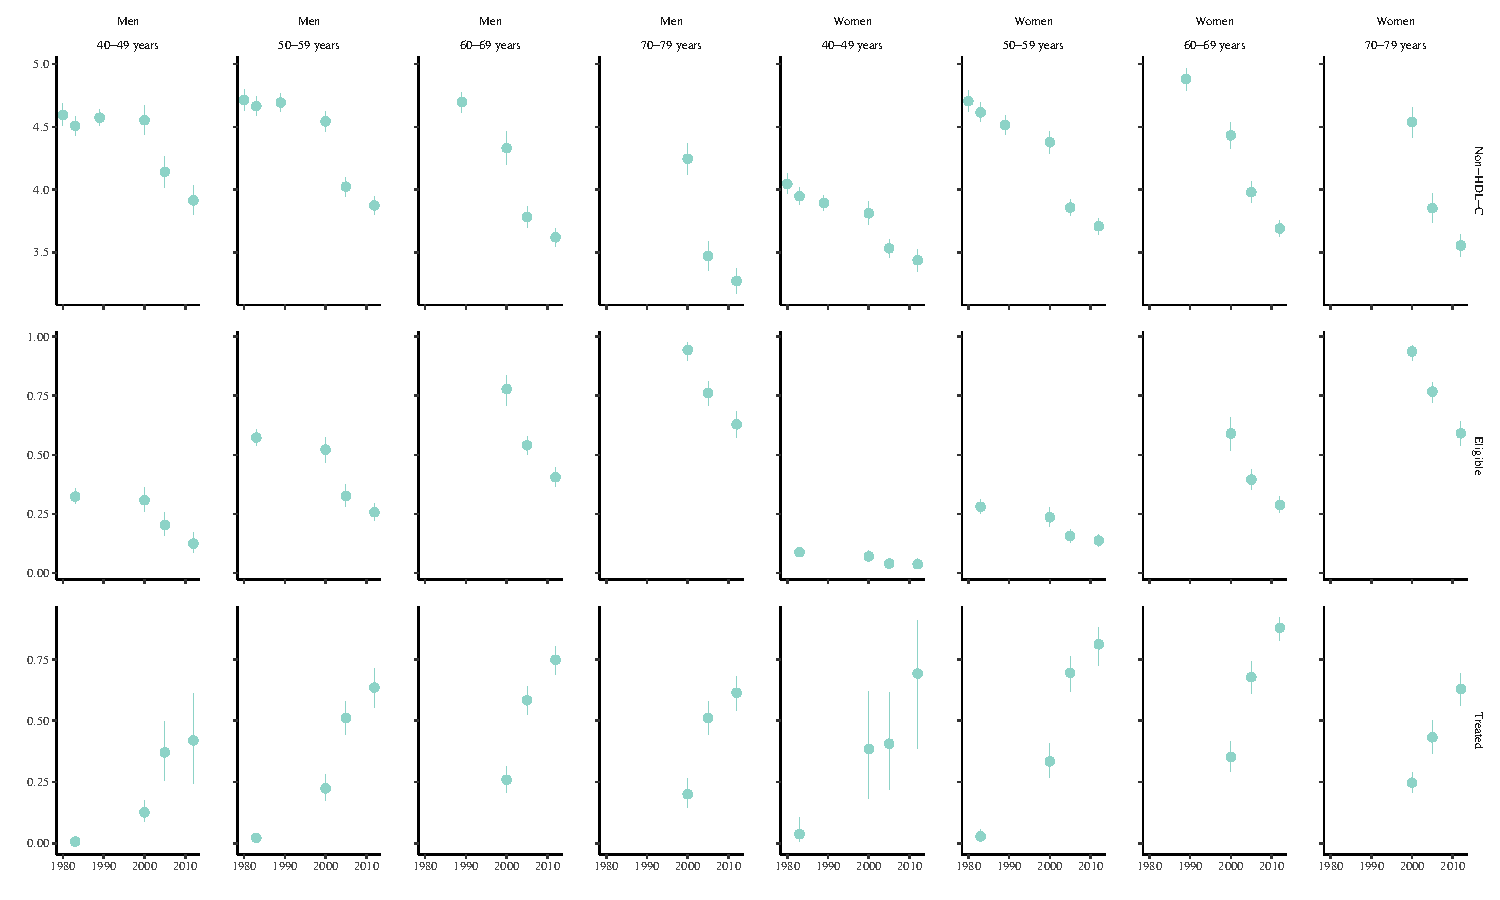
\includegraphics[width=\linewidth]{../3_figures/countries/fig_australia.pdf}
            \caption{Australia}
            \label{fig:australia}
        \end{figure}
    
        \begin{figure}[H]
            \centering
            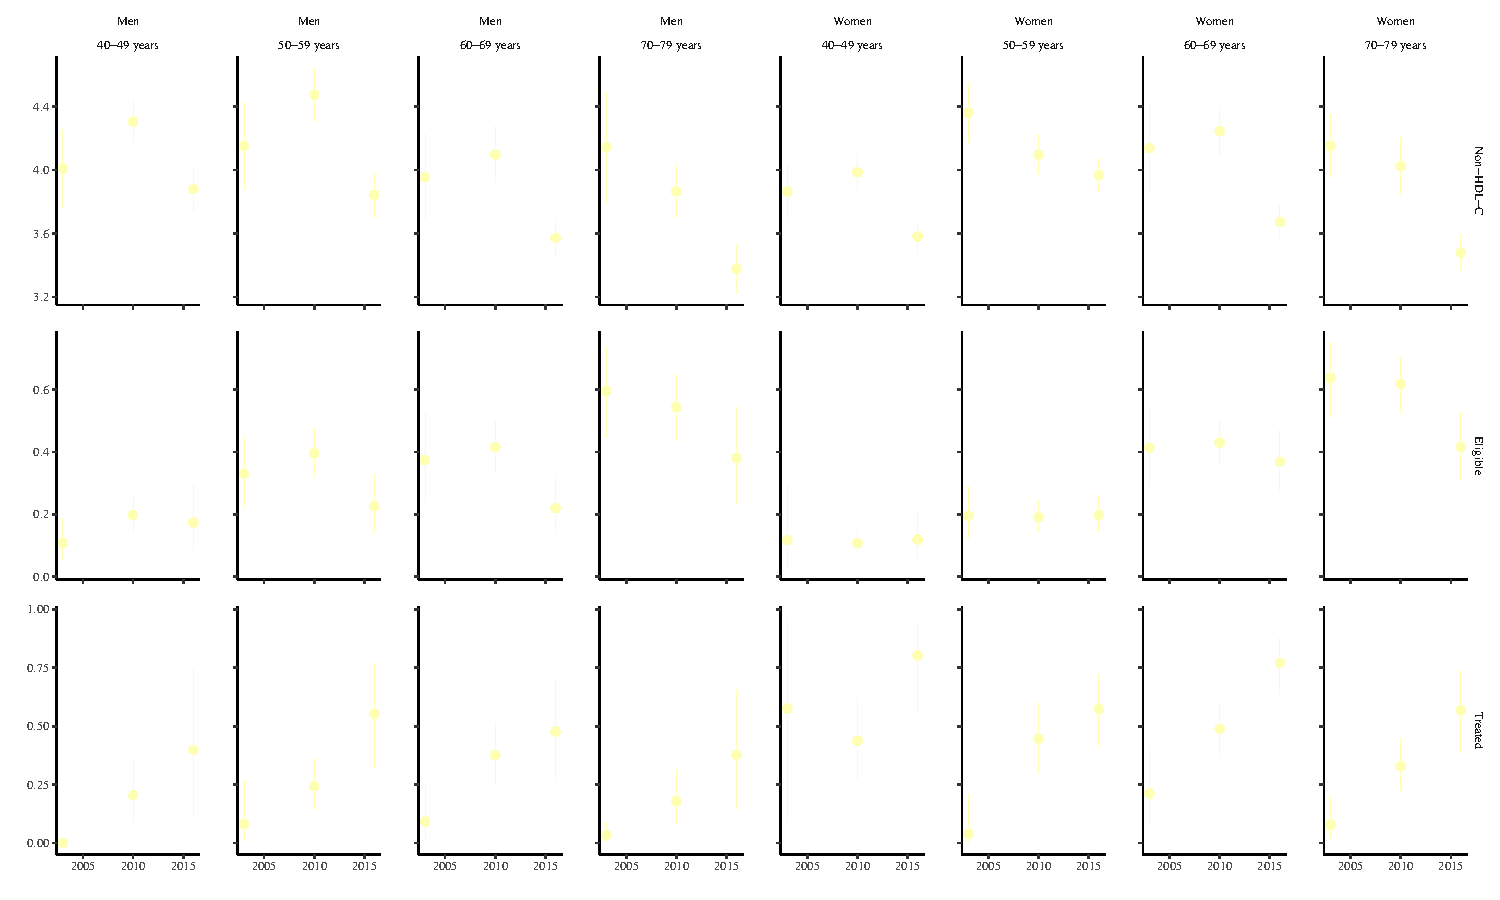
\includegraphics[width=\linewidth]{../3_figures/countries/fig_chile.pdf}
            \caption{Chile}
            \label{fig:chile}
        \end{figure}
    
        \begin{figure}[H]
            \centering
            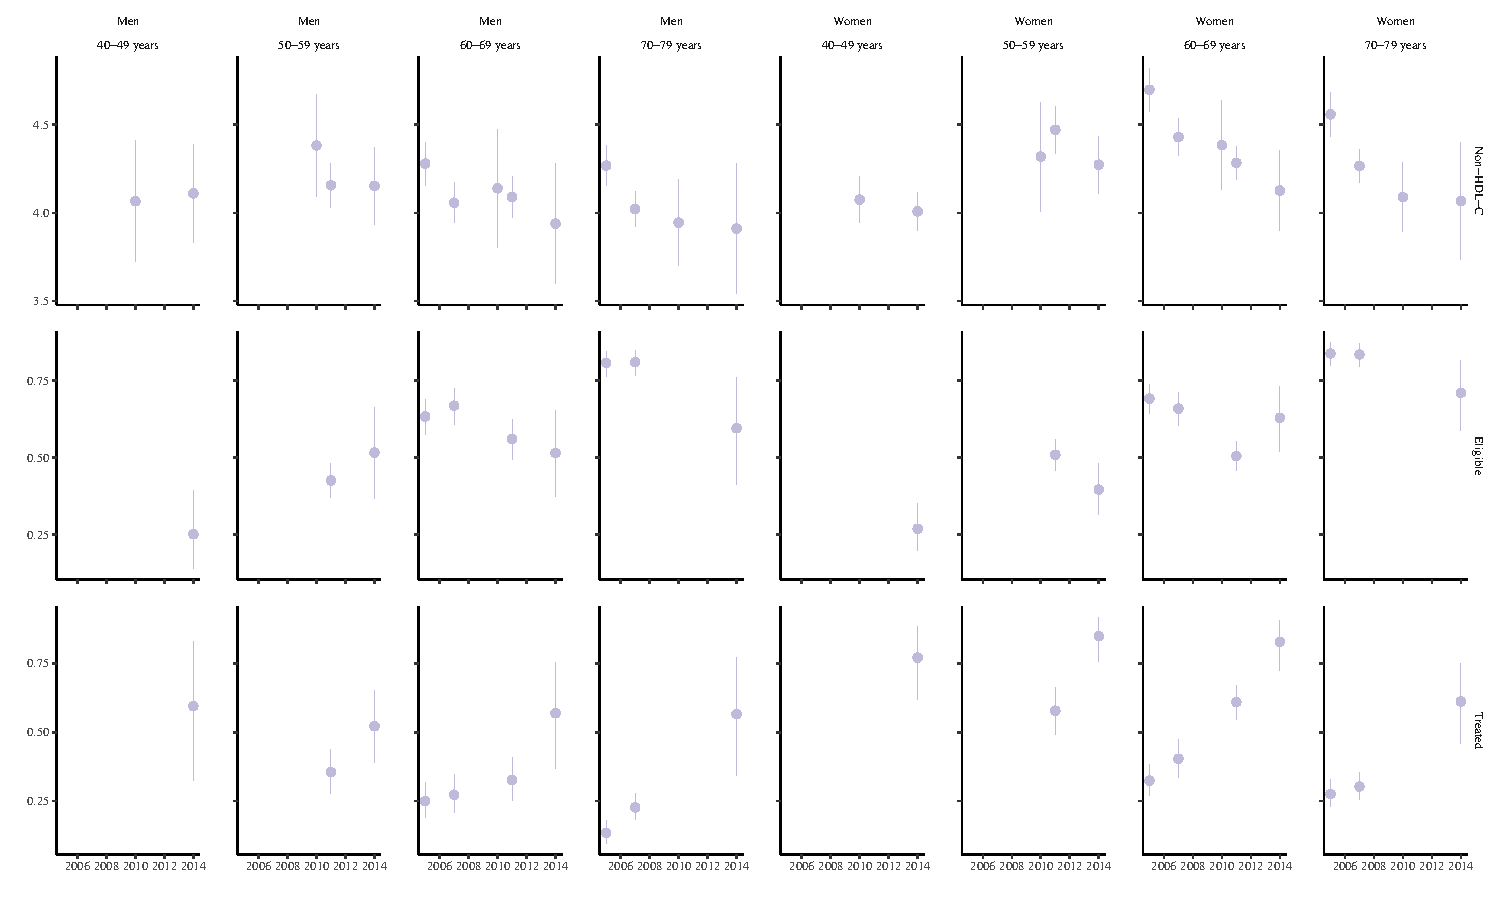
\includegraphics[width=\linewidth]{../3_figures/countries/fig_costa rica.pdf}
            \caption{Costa Rica}
            \label{fig:costa_rica}
        \end{figure}
    
        \begin{figure}[H]
            \centering
            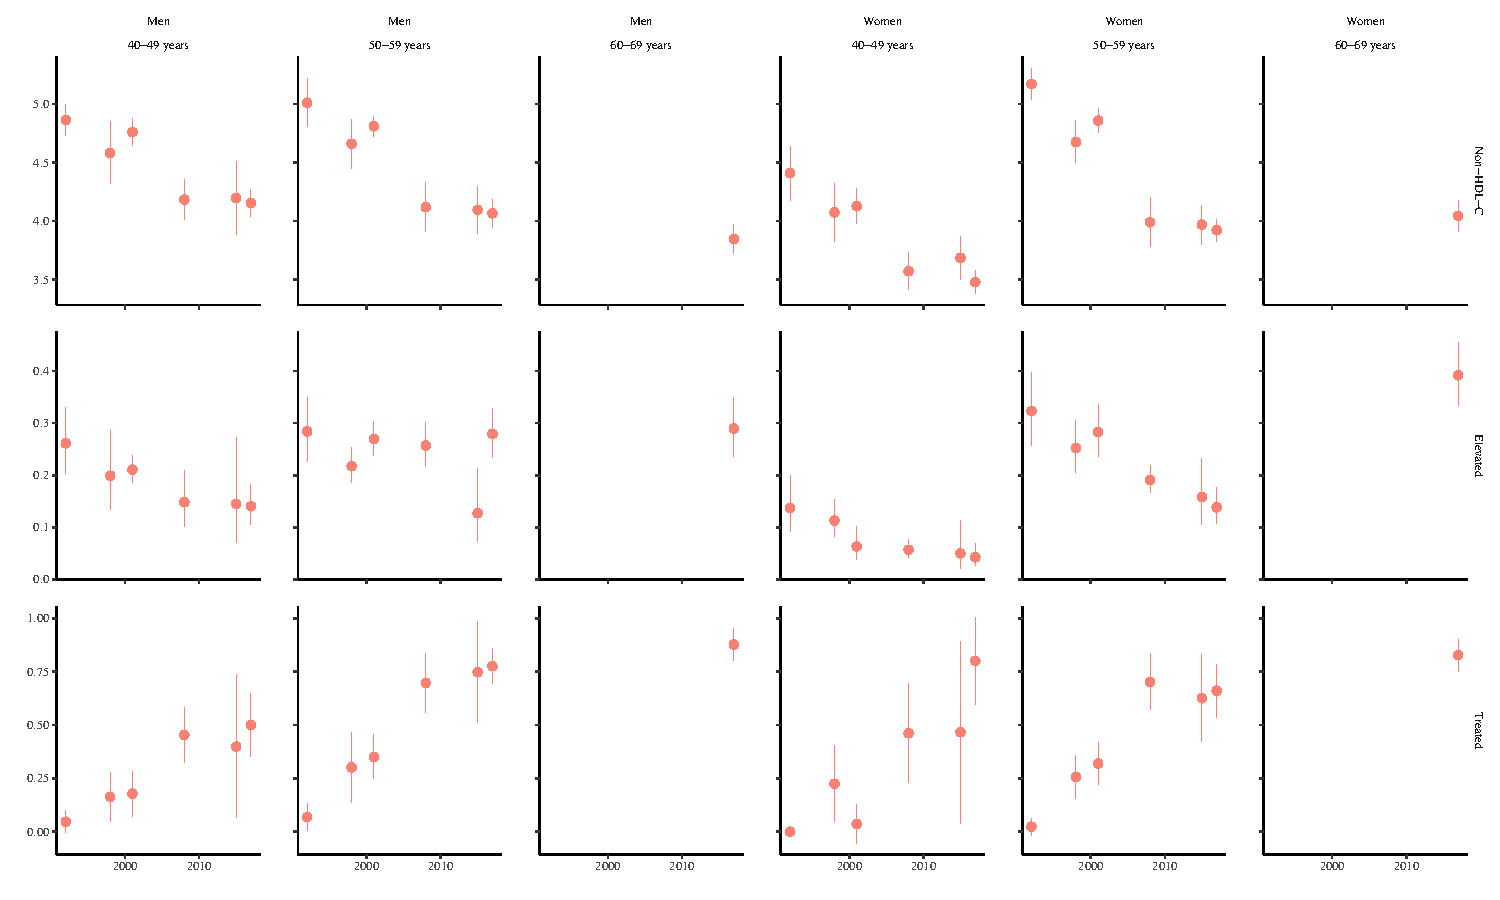
\includegraphics[width=\linewidth]{../3_figures/countries/fig_czechia.pdf}
            \caption{Czechia}
            \label{fig:czechia}
        \end{figure}

        \begin{figure}[H]
            \centering
            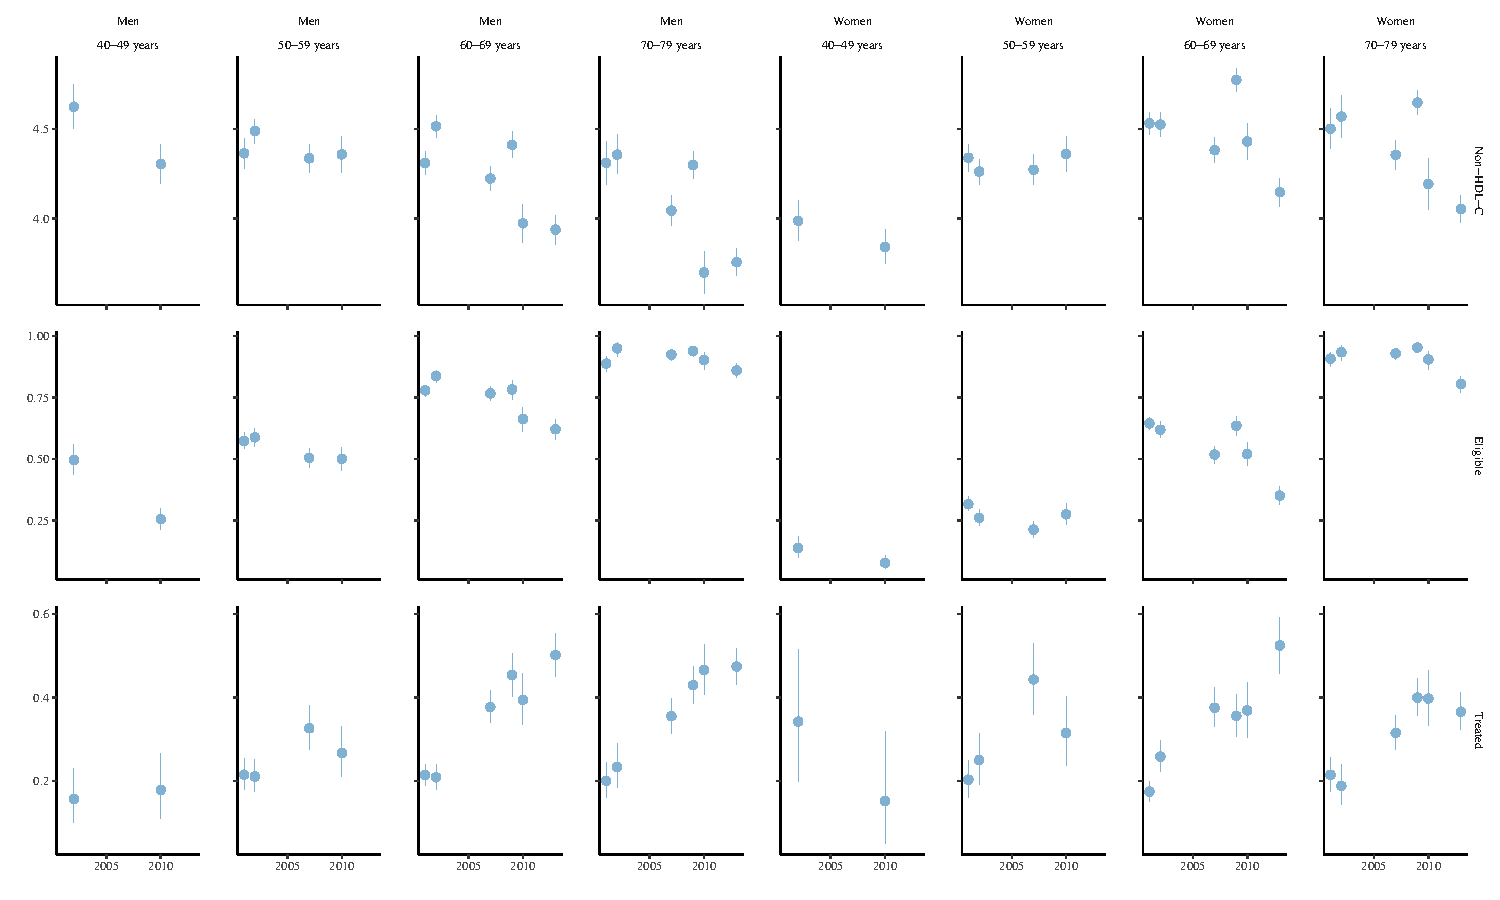
\includegraphics[width=\linewidth]{../3_figures/countries/fig_germany.pdf}
            \caption{Germany}
            \label{fig:germany}
        \end{figure}

        \begin{figure}[H]
            \centering
            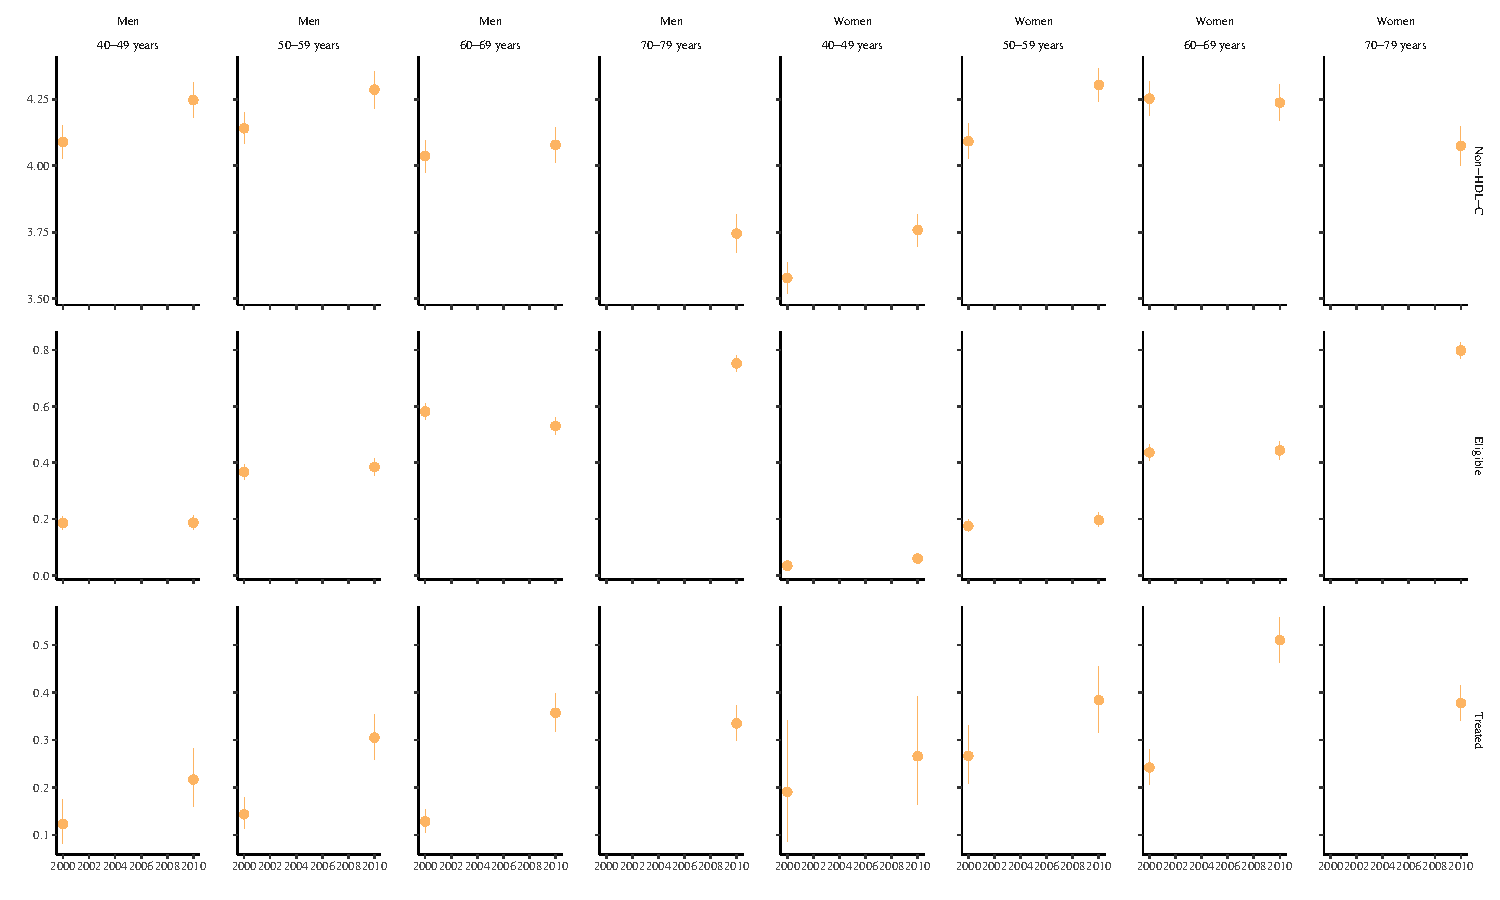
\includegraphics[width=\linewidth]{../3_figures/countries/fig_italy.pdf}
            \caption{Italy}
            \label{fig:italy}
        \end{figure}

        \begin{figure}[H]
            \centering
            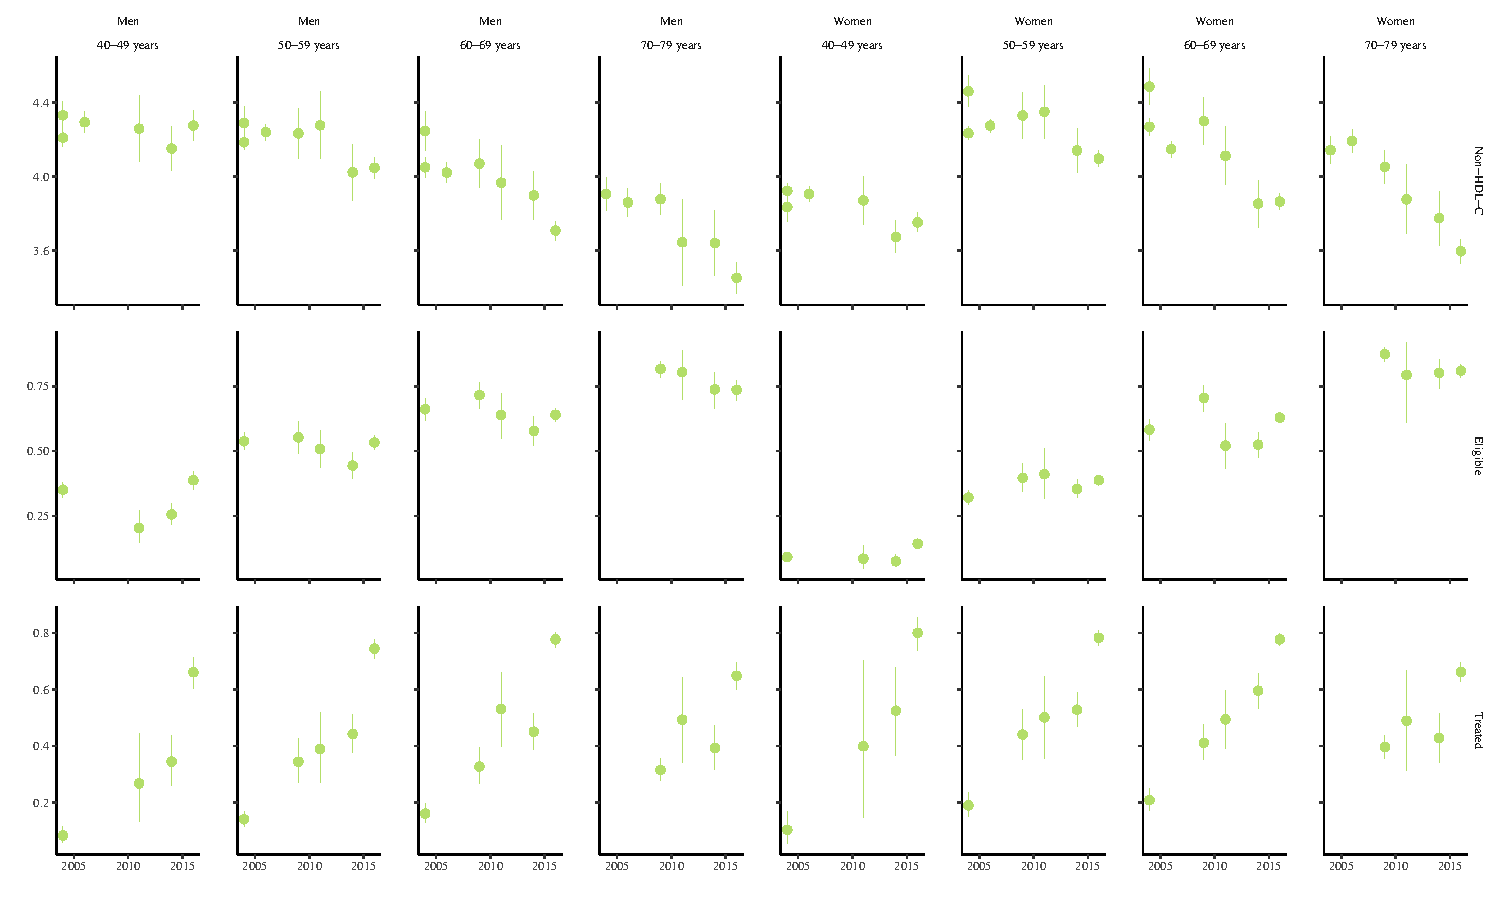
\includegraphics[width=\linewidth]{../3_figures/countries/fig_poland.pdf}
            \caption{Poland}
            \label{fig:poland}
        \end{figure}

        \begin{figure}[H]
            \centering
            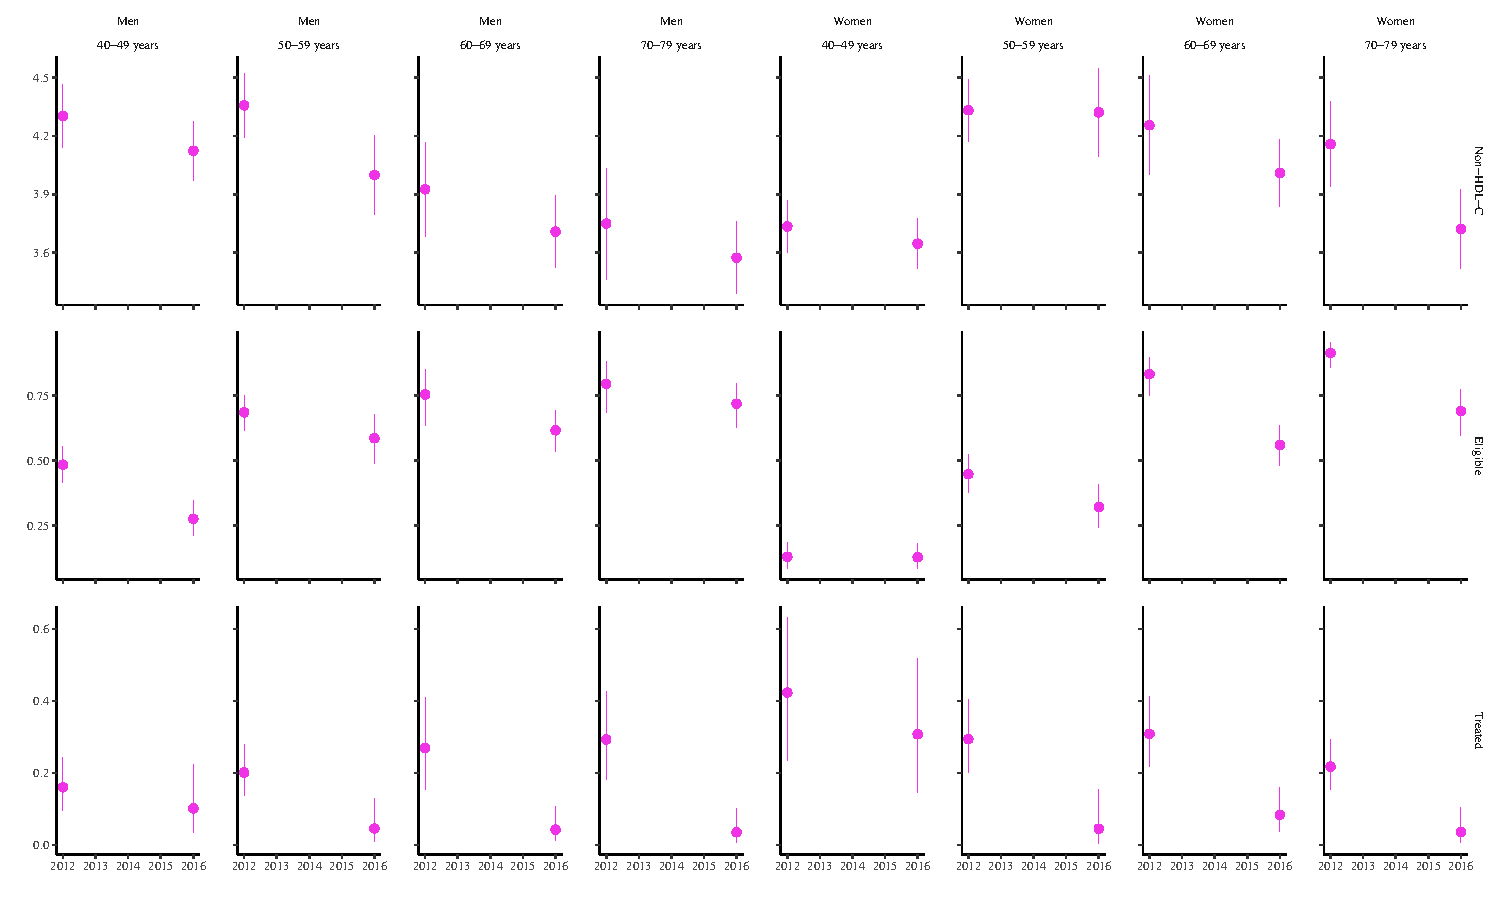
\includegraphics[width=\linewidth]{../3_figures/countries/fig_romania.pdf}
            \caption{Romania}
            \label{fig:romania}
        \end{figure}

        \begin{figure}[H]
            \centering
            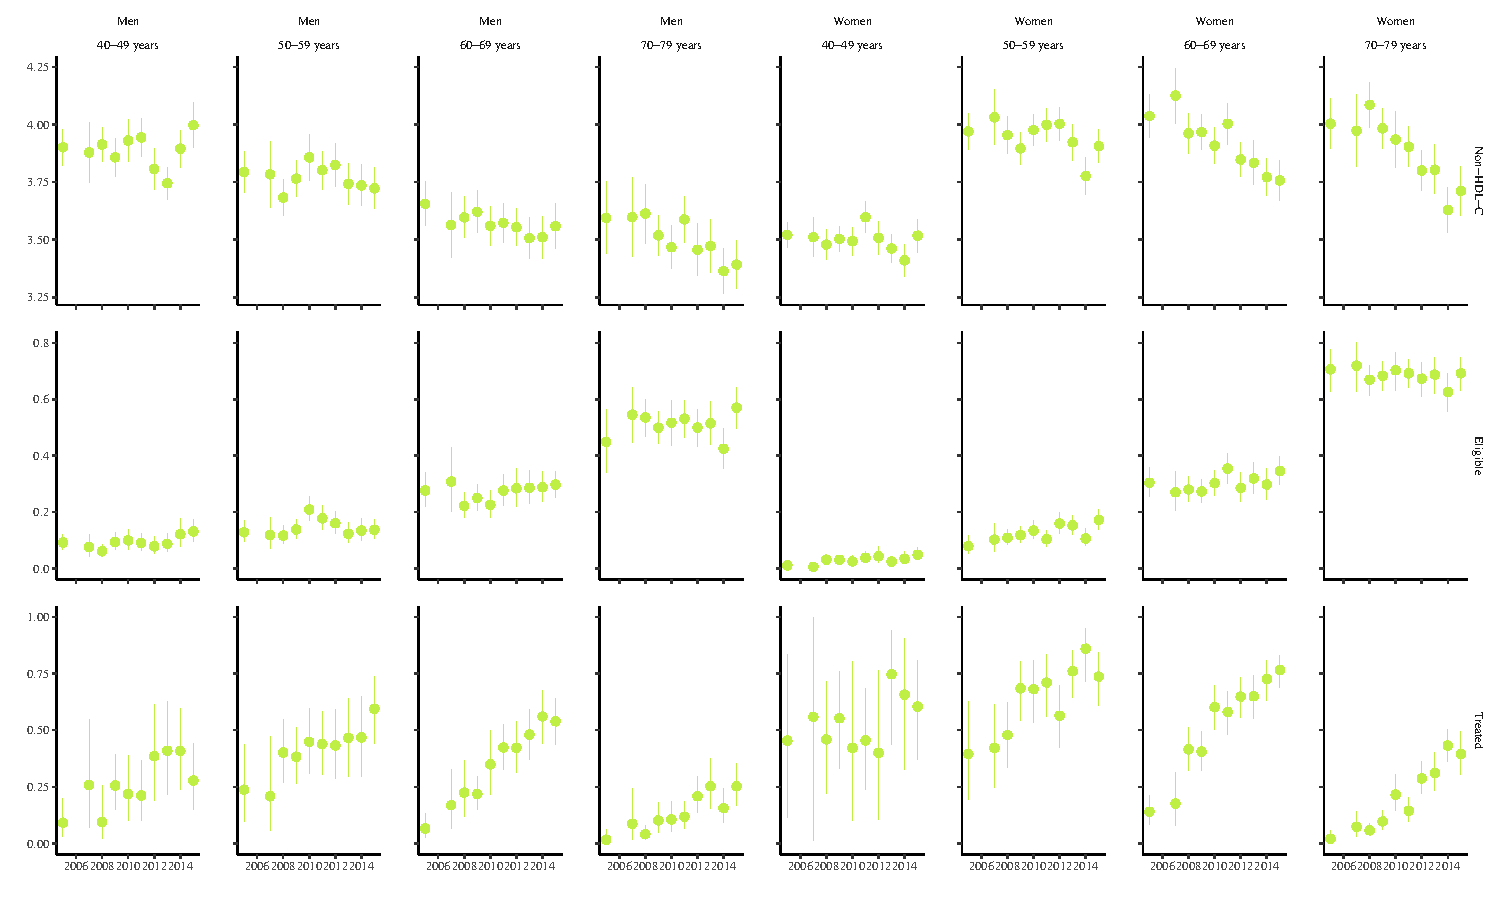
\includegraphics[width=\linewidth]{../3_figures/countries/fig_south korea.pdf}
            \caption{South Korea}
            \label{fig:korea}
        \end{figure}

        \begin{figure}[H]
            \centering
            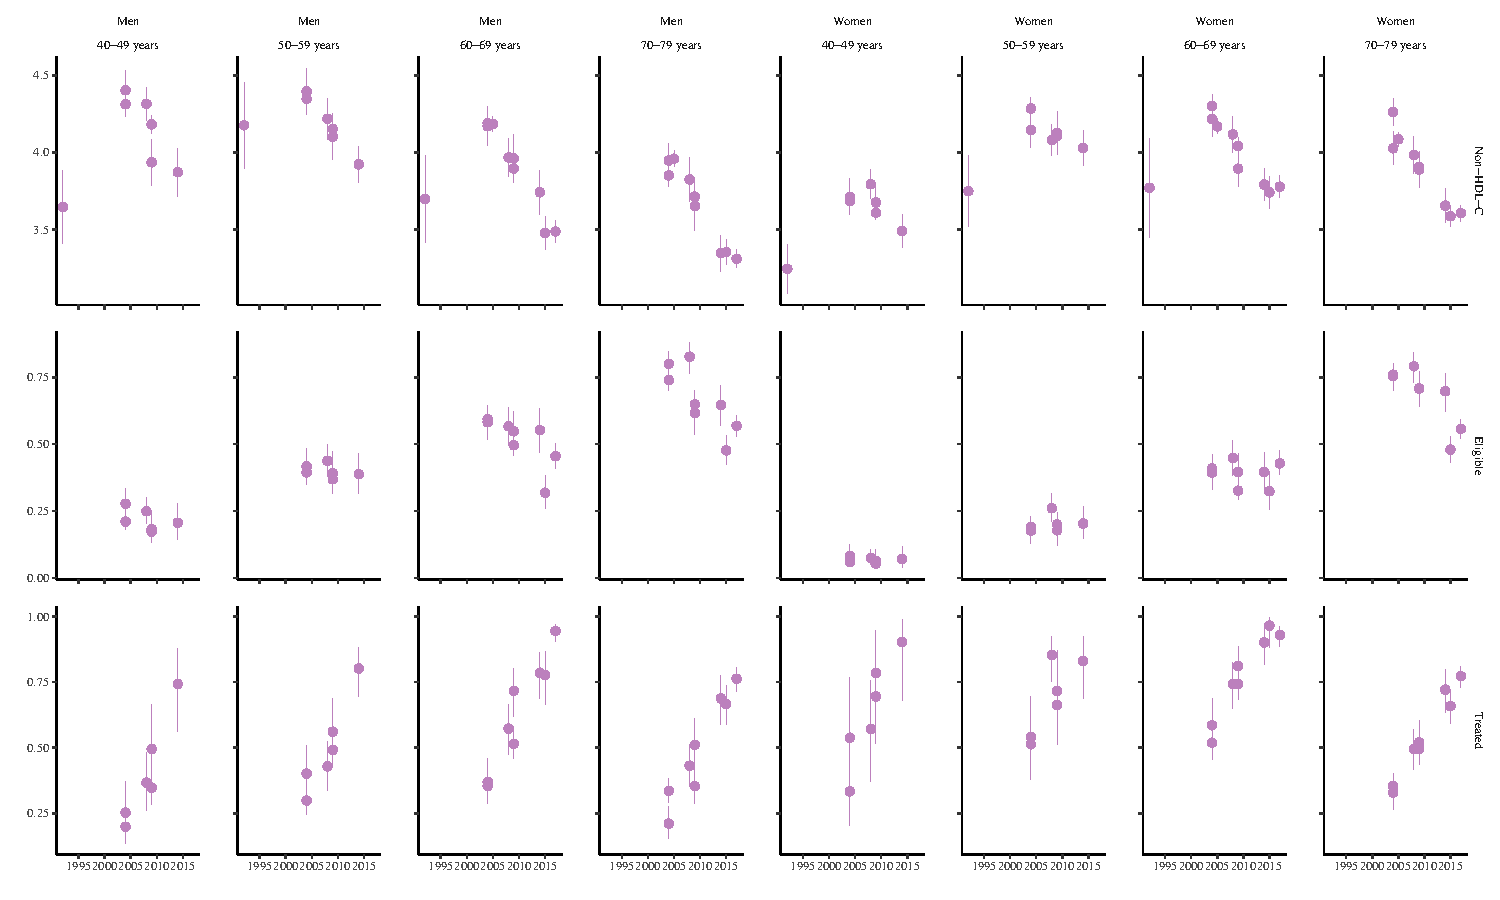
\includegraphics[width=\linewidth]{../3_figures/countries/fig_spain.pdf}
            \caption{Spain}
            \label{fig:spain}
        \end{figure}

        \begin{figure}[H]
            \centering
            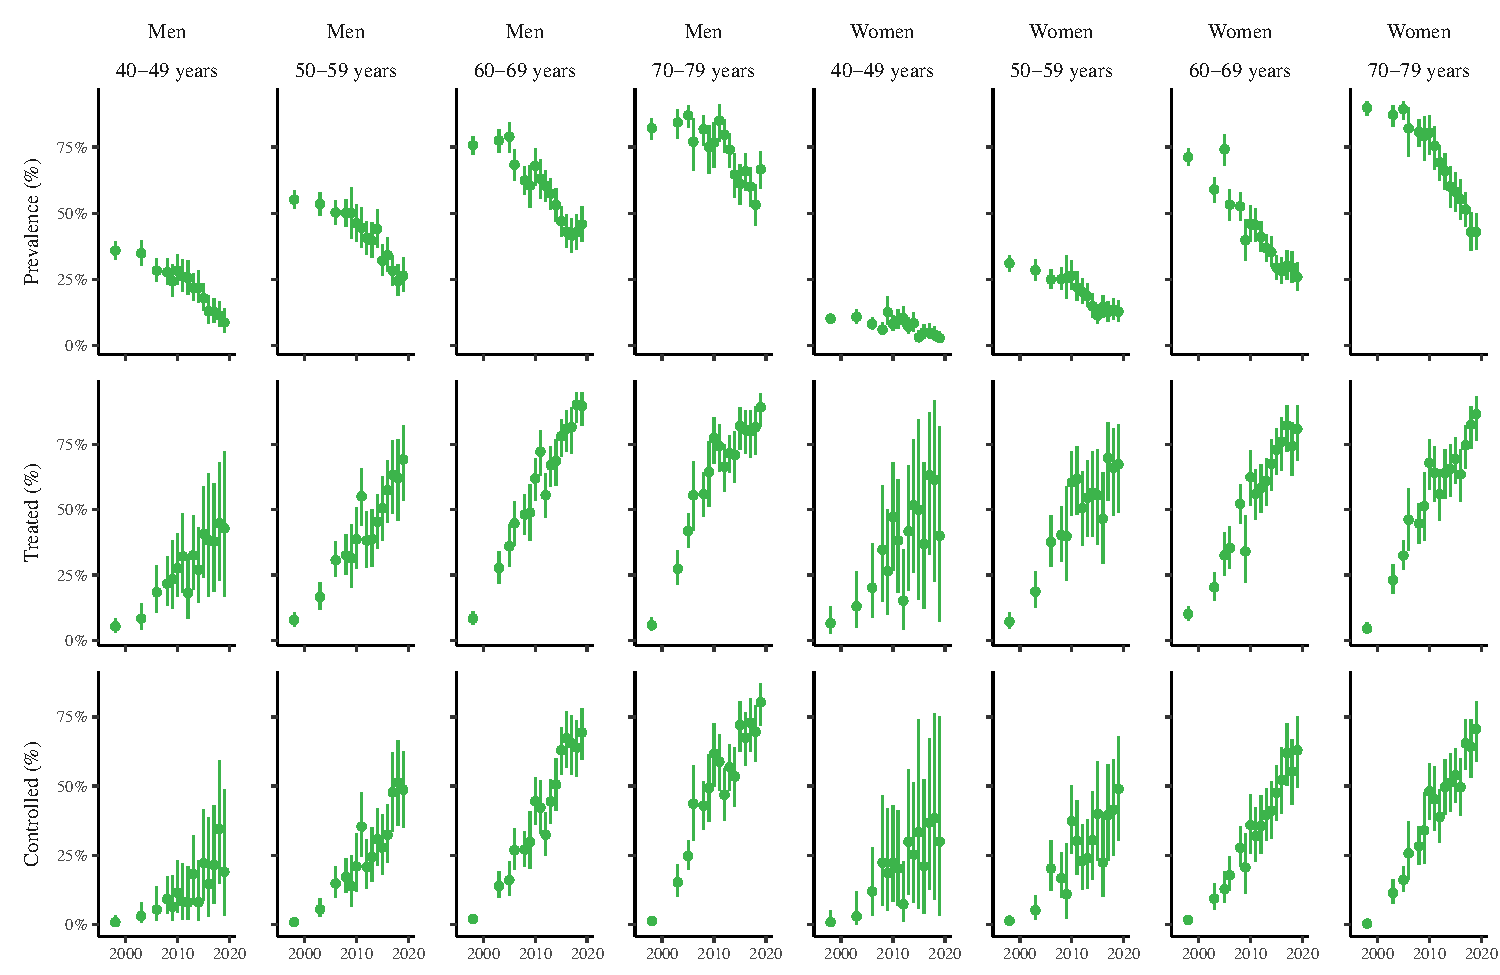
\includegraphics[width=\linewidth]{../3_figures/countries/fig_united kingdom.pdf}
            \caption{United Kingdom}
            \label{fig:uk}
        \end{figure}

        \begin{figure}[H]
            \centering
            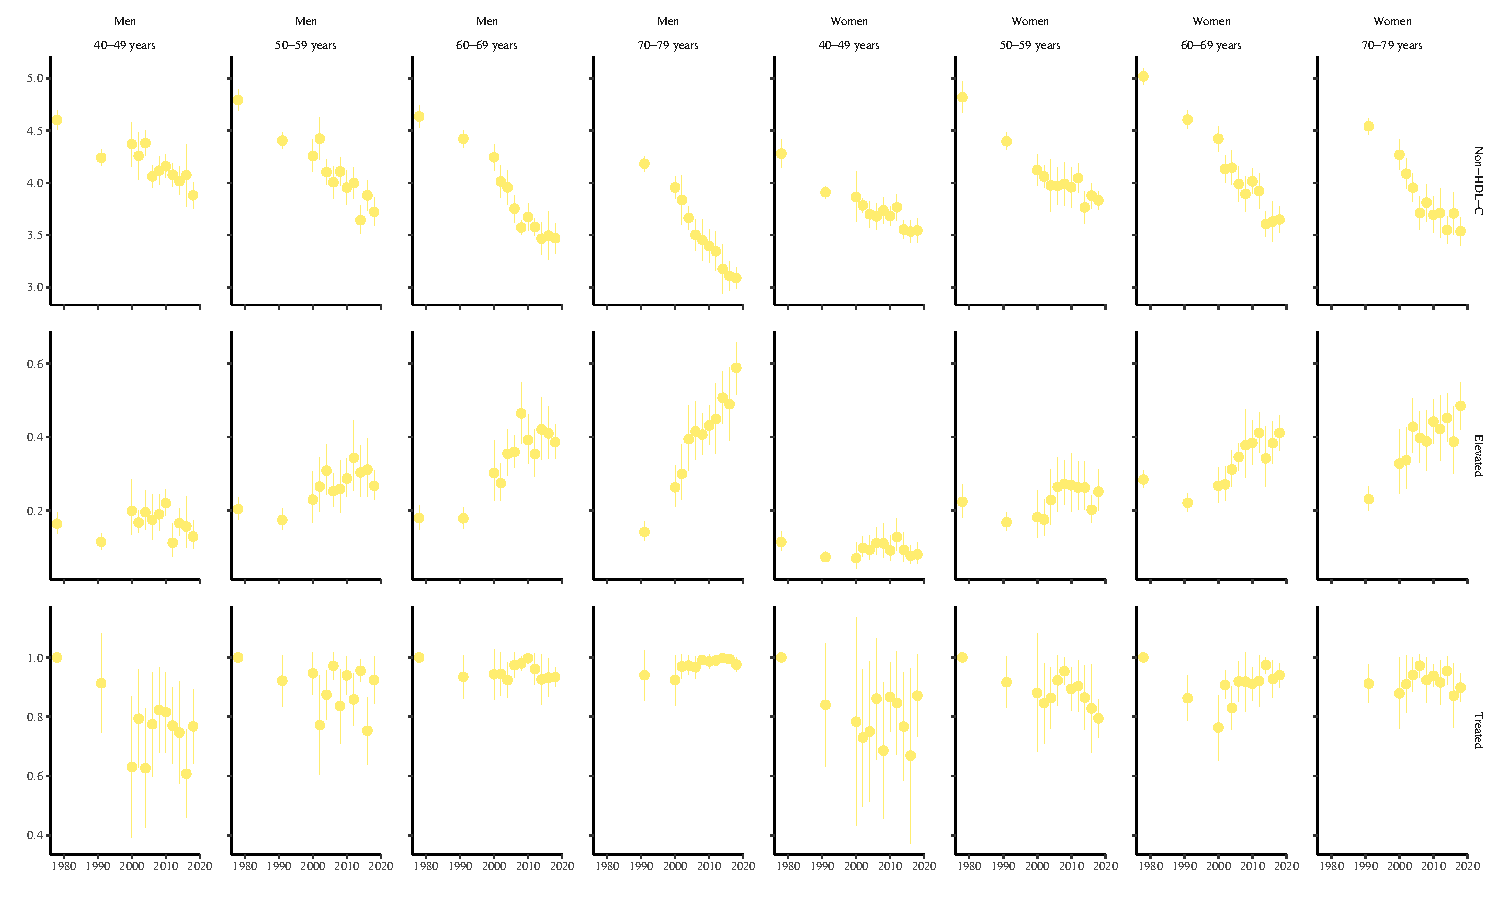
\includegraphics[width=\linewidth]{../3_figures/countries/fig_united states of america.pdf}
            \caption{United States of America}
            \label{fig:usa}
        \end{figure}
    \end{landscape}


    %\printbibliography
    %\bibliography{Placeholder}
\end{appendix}

%\printbibliography

\end{document}